\documentclass[12pt,letterpaper,oneside]{report}

% !TEX root = main.tex
% Codificación, idioma y tipografía
\usepackage[utf8]{inputenc}
\usepackage[T1]{fontenc}
\usepackage[spanish,es-tabla]{babel}
\usepackage{lmodern}
\usepackage{microtype}

% Márgenes solicitados para la plantilla.
% Ajustar únicamente si la universidad entrega medidas institucionales distintas.
\usepackage[
  letterpaper,
  top=2.5cm,
  bottom=2.5cm,
  left=3.0cm,
  right=2.5cm,
  headheight=15pt
]{geometry}

% Interlineado y párrafos
\usepackage{setspace}
\onehalfspacing
\setlength{\parindent}{1.25cm}
\setlength{\parskip}{0pt}

% Figuras, tablas y fórmulas
\usepackage{graphicx}
\graphicspath{{figuras/}}
\usepackage{booktabs}
\usepackage{longtable}
\usepackage{array}
\usepackage{tabularx}
\usepackage{ragged2e}
\usepackage{float}
\usepackage{pdflscape}
\usepackage{amsmath}
\usepackage{amssymb}
\usepackage{caption}
\usepackage{xcolor}
\usepackage{enumitem}

% Enlaces y referencias internas
\usepackage[hidelinks]{hyperref}
\hypersetup{
  pdftitle={Diseño de una arquitectura multiagente para la generación estructurada de artefactos de ingeniería de requisitos},
  pdfauthor={Carvajal Arias, Jhustyn Christopher},
  pdfsubject={Trabajo de titulación},
  pdfkeywords={ingeniería de requisitos, sistemas multiagente, RAG, trazabilidad}
}

% Ajustes generales
\setcounter{secnumdepth}{3}
\setcounter{tocdepth}{3}
\renewcommand{\bibname}{Referencias}
\renewcommand{\contentsname}{Índice general}
\renewcommand{\listfigurename}{Índice de figuras}
\renewcommand{\listtablename}{Índice de tablas}
\captionsetup{font=small,labelfont=bf}
\setlist[itemize]{topsep=3pt,itemsep=2pt,parsep=0pt}
\setlist[enumerate]{topsep=3pt,itemsep=2pt,parsep=0pt}
\newcolumntype{Y}{>{\RaggedRight\arraybackslash}X}
\newcommand{\codigo}[1]{\texttt{\detokenize{#1}}}
\newcommand{\pendiente}[1]{\textcolor{red!70!black}{[Pendiente: #1]}}

% !TEX root = main.tex
\newcommand{\universidad}{Universidad de Cuenca}
\newcommand{\facultad}{Facultad de Ingeniería}
\newcommand{\carrera}{Ingeniería en Ciencias de la Computación}
\newcommand{\tituloTesis}{Diseño de una arquitectura multiagente para la generación estructurada de artefactos de ingeniería de requisitos desde fuentes heterogéneas no estructuradas}
\newcommand{\autorTesis}{Carvajal Arias Jhustyn Christopher}
\newcommand{\tutoraTesis}{Ing. Ana Gabriela Núñez}
\newcommand{\modalidadTesis}{Propuesta tecnológica}
\newcommand{\ciudadTesis}{Cuenca, Ecuador}
\newcommand{\anioTesis}{2026}


\begin{document}

\pagenumbering{roman}
\begin{titlepage}
  \centering
  {\Large\bfseries \universidad\par}
  \vspace{0.7cm}
  {\large\bfseries \facultad\par}
  \vspace{0.3cm}
  {\large \carrera\par}

  \vfill

  {\Large\bfseries \tituloTesis\par}

  \vfill

  {\large Trabajo de titulación previo a la obtención del título correspondiente a la carrera\par}
  \vspace{0.6cm}
  {\large Modalidad: \modalidadTesis\par}

  \vspace{1.2cm}
  \begin{tabular}{rl}
    \textbf{Autor:} & \autorTesis \\
    \textbf{Tutora:} & \tutoraTesis
  \end{tabular}

  \vfill

  {\large \ciudadTesis\par}
  {\large \anioTesis\par}
\end{titlepage}


\clearpage
\tableofcontents
\clearpage
\listoffigures
\clearpage
\listoftables

\clearpage
\pagenumbering{arabic}
\setcounter{page}{1}

% !TEX root = ../main.tex
\chapter{Introducción}
\label{cap:introduccion}

\section{Contexto}

La ingeniería de requisitos constituye una actividad esencial del desarrollo de software porque permite identificar, analizar, documentar y validar las necesidades que deberá satisfacer una solución. Los errores introducidos en esta etapa pueden propagarse hacia el diseño, la implementación y las pruebas, ocasionando retrabajo, aumento de costos e inconsistencias funcionales \cite{sommerville2011}.

En proyectos pequeños y medianos, la información necesaria para definir el sistema suele encontrarse distribuida en entrevistas, reuniones, correos electrónicos, notas, procedimientos y reglas de negocio. Estas fuentes cumplen propósitos diferentes, emplean vocabularios distintos y presentan niveles desiguales de detalle. Por ello, antes de convertirse en requisitos, pueden contener redundancias, omisiones, contradicciones y expresiones ambiguas \cite{wagner2019,palomares2021}.

Los modelos extensos de lenguaje han comenzado a utilizarse para apoyar tareas de obtención, clasificación, reformulación y generación de requisitos. Sin embargo, su capacidad generativa no garantiza que una salida sea correcta para un proyecto concreto. Entre los problemas reportados se encuentran la introducción de información no respaldada, la sensibilidad a la forma del \emph{prompt}, las dificultades con contextos extensos y la falta de mecanismos claros para justificar cada salida \cite{norheim2024,liu2024}.

La recuperación aumentada por generación (\emph{Retrieval-Augmented Generation}, RAG) permite seleccionar fragmentos pertinentes desde una memoria externa y suministrarlos como contexto al modelo \cite{lewis2020}. Por otra parte, una arquitectura multiagente permite separar responsabilidades como ingesta, recuperación, generación, trazabilidad y verificación. La combinación de ambos enfoques ofrece una alternativa para organizar el procesamiento, pero no debe suponerse superior sin evaluación. La tesis estudia una arquitectura concreta y acotada, adecuada al problema y al plazo disponible.

\section{Planteamiento del problema}

La transformación manual de fuentes textuales heterogéneas en artefactos de ingeniería de requisitos demanda que el analista localice información relevante, distinga necesidades de contexto, consolide declaraciones equivalentes, detecte contradicciones y redacte productos verificables. Además, debe conservar el vínculo entre cada artefacto y las fuentes que lo originaron. Esta procedencia previa a la especificación recibe menos atención que la trazabilidad entre requisitos ya escritos y artefactos posteriores del desarrollo \cite{mucha2024}.

Las soluciones recientes basadas en LLM muestran resultados prometedores, pero buena parte de los trabajos cercanos parte de una descripción breve del proyecto, genera un único tipo de artefacto o evalúa enlaces entre artefactos que ya existen. Permanece insuficientemente evaluado un flujo reproducible que procese múltiples géneros textuales de un mismo proyecto, genere requisitos funcionales, requisitos no funcionales e historias de usuario, y conserve evidencia verificable a nivel de fragmento.

En consecuencia, el problema abordado se formula de la siguiente manera: ¿cómo diseñar e implementar una arquitectura multiagente que transforme fuentes textuales heterogéneas en artefactos estructurados de requisitos y mantenga trazabilidad verificable hacia sus fragmentos de origen?

\section{Justificación}

La propuesta tiene relevancia práctica porque busca reducir el esfuerzo de organización inicial sin sustituir la revisión del analista. Los productos generados se consideran propuestas inspeccionables: cada requisito o historia debe incluir identificadores de fragmentos fuente, y las inconsistencias deben registrarse como alertas en lugar de resolverse silenciosamente.

La relevancia académica se encuentra en la definición explícita del proceso y en su evaluación. La tesis no pretende demostrar que una arquitectura sea la mejor de manera universal ni comparar múltiples modelos de lenguaje. Se selecciona una arquitectura orientada por separación de responsabilidades, trazabilidad, reproducibilidad y viabilidad. Su desempeño será evaluado en un caso sintético controlado y comparado con una línea base manual mediante métricas automáticas y juicio de expertos.

\section{Objetivos}

\subsection{Objetivo general}

Desarrollar una arquitectura multiagente para la generación estructurada de requisitos funcionales, requisitos no funcionales e historias de usuario a partir de fuentes textuales heterogéneas y no estructuradas, incorporando mecanismos de recuperación contextual y trazabilidad entre los artefactos generados y sus fuentes originales.

\subsection{Objetivos específicos}

\begin{enumerate}
  \item Diseñar la arquitectura multiagente del sistema, definiendo los agentes, roles, flujos de información y mecanismos de interacción necesarios para el procesamiento estructurado de información textual no estructurada.
  \item Definir el proceso de transformación de fuentes textuales en requisitos funcionales, requisitos no funcionales e historias de usuario, especificando etapas de segmentación, recuperación contextual, generación, trazabilidad, validación y verificación de consistencia.
  \item Implementar un prototipo funcional basado en la arquitectura propuesta, capaz de procesar documentos textuales y entrevistas transcritas mediante mecanismos de recuperación aumentada de información (RAG) y generación asistida por múltiples agentes.
  \item Evaluar el desempeño del prototipo mediante un experimento comparativo frente a una línea base de generación manual de requisitos, analizando criterios de coherencia, completitud, trazabilidad y calidad de los artefactos generados mediante métricas automáticas y juicio de expertos.
\end{enumerate}

\section{Alcance y delimitaciones}

El núcleo de la tesis comprende el diseño de la arquitectura, la definición del proceso, la implementación de un prototipo web y su evaluación frente a una línea base manual. El prototipo admite archivos PDF con texto seleccionable, DOCX, TXT y Markdown, además de fuentes pegadas como texto libre. No exige encabezados ni una plantilla documental previa: los identificadores y fragmentos de trazabilidad se generan durante la ingesta. La transcripción de audio y el reconocimiento óptico de caracteres quedan fuera del alcance actual.

La arquitectura es genérica respecto del dominio. El caso sintético definitivo, denominado SIGSAT, representa la gestión de solicitudes de asistencia técnica y órdenes de trabajo de una organización ficticia de mantenimiento. Sus actores, reglas y decisiones no se encuentran codificados en el núcleo. Cada proyecto obtiene su contexto únicamente de los metadatos declarados por el usuario, sus fuentes y las respuestas confirmadas durante la etapa de definición. El corpus combina quince fuentes sintéticas con una resolución pública ecuatoriana de protección de datos, sin incorporar información personal real.

La evaluación principal compara el tratamiento multiagente con la producción manual usando el mismo corpus, la misma definición confirmada del proyecto y la misma guía de artefactos. Un agente único con RAG y un conjunto adjudicado de referencia podrán incorporarse como extensiones si el cronograma y la disponibilidad de evaluadores lo permiten; no constituyen condiciones necesarias para cumplir los objetivos aprobados. La calidad final será determinada mediante evidencia automática y juicio experto, sin formular una hipótesis direccional que obligue al sistema a superar la línea base.

\section{Estructura del documento}

El Capítulo~\ref{cap:estado-arte} presenta los antecedentes. El Capítulo~\ref{cap:marco-teorico} define los conceptos centrales. El Capítulo~\ref{cap:metodologia} describe el diseño metodológico. Los capítulos~\ref{cap:arquitectura} y~\ref{cap:proceso} desarrollan los objetivos específicos 1 y 2. El Capítulo~\ref{cap:implementacion} documenta el prototipo, mientras que el Capítulo~\ref{cap:evaluacion} reunirá el experimento y sus resultados. Finalmente, el Capítulo~\ref{cap:conclusiones} presentará conclusiones, limitaciones y trabajo futuro.

% !TEX root = ../main.tex
\chapter{Estado del arte}
\label{cap:estado-arte}

\section{Alcance y procedimiento de revisión}

Se realizó una revisión estructurada del corpus bibliográfico disponible para la tesis. Fueron abiertos y clasificados 47 documentos, con lectura profunda de los trabajos directamente comparables y lectura dirigida de las fuentes de apoyo. La revisión consideró combinaciones de los términos \emph{requirements engineering}, \emph{large language model}, \emph{multi-agent}, RAG, \emph{traceability}, \emph{provenance}, \emph{unstructured documents} y \emph{user stories}.

La búsqueda priorizó artículos revisados por pares, capítulos académicos, normas y páginas oficiales. Los preprints se conservaron cuando no se identificó una versión publicada. Este procedimiento permite construir un estado del arte trazable, pero no se presenta como una nueva revisión sistemática exhaustiva de todas las bases. En consecuencia, se evitan afirmaciones absolutas de prioridad y se conserva un protocolo para actualizar la búsqueda antes de la entrega final.

\begin{table}[H]
  \centering
  \caption{Criterios aplicados en la revisión del estado del arte}
  \label{tab:criterios-revision}
  \small
  \begin{tabularx}{\textwidth}{>{\bfseries}p{0.24\textwidth}Y}
    \toprule
    Elemento & Definición aplicada \\
    \midrule
    Pregunta & ¿Qué entradas, salidas, arquitecturas, mecanismos de recuperación, trazas, líneas base y métricas utilizan los estudios cercanos? \\
    Ventana & NLP y trazabilidad desde 2015; LLM y agentes desde 2020; fundamentos sin límite temporal cuando son necesarios. \\
    Inclusión & Estudios con método y resultados verificables que extraen, generan, transforman, validan o enlazan artefactos de requisitos. \\
    Exclusión & Generación de código sin tarea de requisitos, ensayos sin evaluación, duplicados y versiones preliminares cuando existe versión publicada. \\
    Campos & Entrada, salida, técnica, agentes, RAG, trazabilidad, evaluación, reproducibilidad, limitaciones y relación con la tesis. \\
    \bottomrule
  \end{tabularx}
\end{table}

\section{Ingeniería de requisitos y fuentes heterogéneas}

La ingeniería de requisitos comprende actividades de obtención, análisis, especificación, validación y gestión de necesidades y requisitos \cite{iso29148,sommerville2011}. En la práctica, la información inicial puede estar distribuida en entrevistas, reuniones, correos, formularios, políticas, incidencias y documentos legados. Los estudios industriales muestran diversidad de técnicas, roles y problemas de comunicación; sus resultados también dependen del contexto organizacional \cite{wagner2019,palomares2021}.

La heterogeneidad relevante para esta tesis no se limita al formato del archivo. Se operacionaliza mediante diferencias de género documental, propósito, autor, temporalidad, vocabulario y nivel de detalle. La diversidad puede producir contradicciones, pero también aporta evidencias complementarias. El desafío consiste en normalizar las necesidades sin eliminar el vínculo con su procedencia.

\section{Trazabilidad previa a la especificación}

La literatura diferencia la trazabilidad posterior a la especificación ---por ejemplo, requisito a diseño, código o prueba--- de la trazabilidad previa. Esta última vincula los requisitos con fuentes como entrevistas, minutas y sistemas legados. La revisión de Mucha, Kaufmann y Riehle muestra que la trazabilidad previa ha recibido menos atención y enfrenta barreras de esfuerzo, mantenimiento y percepción de utilidad \cite{mucha2024}.

Los modelos preentrenados han ampliado la recuperación semántica de enlaces y el procesamiento de lenguaje natural ofrece técnicas para localizar relaciones entre artefactos \cite{guo2025}. Sin embargo, enlazar dos artefactos existentes no equivale a conservar evidencia mientras se genera uno nuevo. Esta diferencia sustenta la procedencia a nivel de fragmento adoptada en la tesis.

\section{Modelos de lenguaje en ingeniería de requisitos}

Los LLM se han aplicado a elicitación asistida, extracción, clasificación, reformulación, verificación y generación de especificaciones. Las revisiones recientes señalan diversidad de entradas, estrategias de \emph{prompting} y métricas, junto con problemas recurrentes de reproducibilidad, alucinación, evaluación e integración humana \cite{hemmat2025,cheng2026}.

El potencial generativo no elimina la necesidad de controles. Norheim et al.\ agrupan dificultades de conocimiento, completitud, procedimiento, entrada, \emph{prompting}, evaluación y formato \cite{norheim2024}. Asimismo, el rendimiento puede disminuir cuando la evidencia relevante se encuentra en posiciones intermedias de contextos extensos \cite{liu2024}. Esto justifica segmentar, recuperar y verificar, sin atribuir a RAG una capacidad automática de resolver información faltante.

\section{Recuperación aumentada y trazabilidad}

RAG combina la memoria paramétrica del modelo generativo con una memoria externa recuperable. El enfoque fundacional condiciona la generación a pasajes seleccionados y hace posible inspeccionar qué información fue recuperada \cite{lewis2020}. En esta tesis, el índice contiene fragmentos de las fuentes del proyecto y, después de la confirmación humana, fragmentos diferenciados de la definición. Las salidas generadas no se incorporan como evidencia documental.

Ali, Naganathan y Bork combinan RAG y LLM para recuperar enlaces entre requisitos y código \cite{ali2024}. QUARE emplea recuperación de cláusulas normativas para verificar modelos de objetivos \cite{quare2026}. Ambos antecedentes muestran que RAG puede apoyar trazabilidad o fundamentación, aunque sus objetos de recuperación difieren de la evidencia documental del proyecto considerada aquí.

\section{Arquitecturas multiagente aplicadas a requisitos}

Una arquitectura multiagente distribuye responsabilidades entre roles y define cómo intercambian artefactos, revisan resultados y controlan la ejecución. MetaGPT ejemplifica el empleo de roles y procedimientos operativos para producir artefactos intermedios \cite{metagpt2024}. No obstante, dividir una tarea no demuestra por sí mismo una ventaja; la arquitectura debe justificarse y evaluarse.

\subsection{MARE}

MARE organiza actividades de elicitación, modelado, verificación y especificación mediante agentes y un espacio compartido de artefactos. Incluye líneas base y una ablación frente a un LLM individual \cite{mare2024}. Su entrada habitual es una idea breve de proyecto; no evalúa la transformación de un paquete documental heterogéneo ni enlaces a fragmentos fuente.

\subsection{Generación y priorización de historias de usuario}

Sami et al.\ emplean roles de Product Owner, QA, Developer y Manager para generar, revisar y priorizar historias de usuario desde una descripción de proyecto \cite{sami2024}. El trabajo respalda la viabilidad de una cadena multiagente, aunque su alcance preliminar no incorpora una evaluación de procedencia documental.

\subsection{iReDev}

iReDev utiliza seis agentes dirigidos por conocimiento, un repositorio de artefactos y puntos de colaboración humana para producir requisitos, modelos y una especificación \cite{iredev2025}. Su registro de qué agente originó un artefacto representa trazabilidad del proceso, pero no identifica el documento y fragmento que respaldan el contenido.

\subsection{Debate multiagente}

Oriol et al.\ aplican participantes y un juez a la clasificación de requisitos funcionales y no funcionales. El debate puede mejorar el desempeño frente a un agente individual, aunque también incrementa tokens y costo \cite{oriol2025}. Este resultado respalda la revisión especializada, pero no demuestra que más agentes mejoren toda tarea de generación.

\subsection{ReqNet}

ReqNet compara múltiples \emph{pipelines} para clasificar oraciones de documentos no estructurados como requisito o no requisito \cite{reqnet2026}. Es relevante para la identificación de información, pero no normaliza necesidades en RF, RNF e historias de usuario ni produce trazabilidad generativa.

\subsection{Generación desde títulos de incidencias}

Paiva, Canedo y Rocha Filho generan requisitos desde títulos de incidencias y evalúan propiedades lingüísticas con apoyo humano \cite{paiva2026}. El estudio distingue acertadamente la buena forma de la corrección contextual: una declaración clara puede seguir siendo incorrecta o incompleta para el dominio.

\subsection{QUARE y TraceLLM}

QUARE coordina agentes especializados y un orquestador, negocia atributos de calidad y emplea RAG normativo \cite{quare2026}. TraceLLM, por su parte, diseña y evalúa \emph{prompts} para recuperar enlaces entre artefactos existentes en varios \emph{benchmarks} \cite{tracellm2026}. El primero recupera normativa y el segundo aborda trazabilidad posterior; ninguno evalúa exactamente la conservación de procedencia durante la generación de RF, RNF e historias desde múltiples fuentes del mismo proyecto.

\section{Comparación de antecedentes directos}

\begin{landscape}
\begin{longtable}{p{2.7cm}p{3.6cm}p{3.7cm}p{4.0cm}p{4.3cm}}
  \caption{Comparación de trabajos directamente relacionados}
  \label{tab:comparacion-antecedentes}\\
  \toprule
  Trabajo & Entrada y salida & Arquitectura & Evaluación & Diferencia respecto de la tesis \\
  \midrule
  \endfirsthead
  \toprule
  Trabajo & Entrada y salida & Arquitectura & Evaluación & Diferencia respecto de la tesis \\
  \midrule
  \endhead
  MARE \cite{mare2024} & Idea breve a modelos y especificación & Cinco agentes; sin RAG documental & Métricas, evaluación humana y líneas base & No procesa corpus heterogéneo ni enlaza fragmentos fuente. \\
  Sami et al.\ \cite{sami2024} & Descripción a historias y prioridad & Cuatro roles; sin RAG & Un proyecto, similitud, tiempo y clasificación & Estudio preliminar sin procedencia documental. \\
  iReDev \cite{iredev2025} & Descripción a requisitos, modelos y SRS & Seis agentes y colaboración humana & Diez casos y métricas automáticas & Registra agente de origen, no evidencia documental. \\
  Debate \cite{oriol2025} & Requisitos existentes a clase RF/RNF & Dos participantes y juez & F1 y comparación con agente único & Clasifica; no genera ni conserva procedencia. \\
  ReqNet \cite{reqnet2026} & Documentos a requisito/no requisito & Múltiples \emph{pipelines}; sin agentes & Conjuntos públicos, precisión, recall y F1 & No produce RF, RNF, HU ni enlaces. \\
  Issue titles \cite{paiva2026} & Título de incidencia a requisito & LLM con estrategias de \emph{prompting} & Calidad lingüística y revisión humana & Entrada mínima; la corrección contextual requiere más evidencia. \\
  QUARE \cite{quare2026} & Descripción a modelos KAOS & Agentes y RAG normativo & Casos, semillas y comparadores & Recupera normas, no fragmentos de las fuentes del proyecto. \\
  TraceLLM \cite{tracellm2026} & Artefactos existentes a enlaces & \emph{Prompting} con varios LLM & \emph{Benchmarks}, precisión, recall, F1 y F2 & Trazabilidad posterior; no genera requisitos. \\
  \bottomrule
\end{longtable}
\end{landscape}

\section{Brecha y posicionamiento}

La combinación general de LLM, RAG, agentes y validación ya aparece en la literatura. Por ello, la contribución no se formula como la simple unión de tecnologías. La brecha operacional se concentra en un flujo que: procesa géneros textuales heterogéneos de un mismo proyecto; genera RF, RNF e historias de usuario; conserva enlaces verificables artefacto--fragmento; registra alertas sin ocultar contradicciones; y compara el resultado con producción manual bajo un caso controlado.

La arquitectura propuesta se presenta como una opción adecuada al problema y no como la mejor arquitectura universal. La tesis deberá demostrar que fue especificada, implementada y evaluada de forma reproducible, incluso si los resultados finales no muestran superioridad sobre la línea base.

% !TEX root = ../main.tex
\chapter{Marco teórico}
\label{cap:marco-teorico}

\section{Ingeniería de requisitos}

La ingeniería de requisitos comprende los procesos mediante los cuales se descubren, analizan, documentan, validan y gestionan las necesidades y restricciones de un sistema. ISO/IEC/IEEE 29148:2018 organiza estas actividades y describe características de requisitos bien formados e ítems de información para su documentación \cite{iso29148}. La norma se utiliza en esta investigación como fundamento de diseño y evaluación, no como declaración de certificación.

\subsection{Necesidad, requisito y artefacto}

Una necesidad expresa una capacidad, problema, restricción o cualidad relevante para un interesado o para el entorno. Un requisito transforma una necesidad en una declaración suficientemente precisa para orientar la solución y permitir su verificación. En esta tesis se denomina \emph{artefacto} a cada salida estructurada: requisito funcional (RF), requisito no funcional (RNF) o historia de usuario (HU).

La transformación no es una paráfrasis mecánica. Puede requerir separar una declaración compuesta, reunir evidencia complementaria, clasificar la información, declarar elementos faltantes y conservar la procedencia. El sistema no debe inventar actores, prioridades, umbrales, beneficios ni criterios de aceptación. Cuando la evidencia sea contradictoria o insuficiente, la decisión debe solicitarse al usuario o el artefacto debe marcarse para aclaración.

\subsection{Requisitos funcionales y no funcionales}

Los RF describen servicios, comportamientos o respuestas que el sistema debe proporcionar. Los RNF expresan cualidades, restricciones o condiciones bajo las cuales se prestan esas funciones. La clasificación depende del significado y del alcance, no únicamente de palabras clave.

En ReqLab, ambos tipos incluyen identificador, título, descripción verificable, prioridad, estado, fragmentos fuente y relaciones con otros artefactos. En el RNF, la redacción debe expresar una propiedad de calidad o restricción susceptible de comprobación. Las alertas automáticas apoyan la revisión, pero la decisión final corresponde al analista.

\subsection{Historias de usuario}

Una historia de usuario representa una necesidad desde la perspectiva de un rol y suele adoptar la estructura ``Como [rol], quiero [objetivo], para [beneficio]''. Su calidad no depende únicamente de respetar la plantilla: debe evitar ambigüedad, conservar una finalidad respaldada y disponer de criterios de aceptación observables \cite{lucassen2016}.

El prototipo comprueba su forma mínima y la existencia de criterios de aceptación. La corrección contextual y la utilidad de la historia se determinan posteriormente mediante revisión humana y juicio experto.

\section{Fuentes textuales heterogéneas}

Una fuente textual es una unidad documental con identidad y procedencia. La heterogeneidad se manifiesta en el tipo de archivo, género, propósito, autor, canal, temporalidad, vocabulario, estructura y grado de formalidad. El corpus puede contener correos copiados, entrevistas transcritas, conversaciones, notas, políticas y documentos narrativos sin una plantilla de requisitos.

ReqLab admite PDF con texto seleccionable, DOCX, TXT y Markdown, además de texto pegado directamente en la interfaz. La extracción transforma el contenedor a texto; no presupone que el contenido ya esté clasificado como RF, RNF o HU. El OCR de imágenes y la transcripción automática de audio quedan fuera del alcance, por lo que un PDF escaneado o una grabación deben convertirse previamente en texto.

\subsection{Fragmento y segmentación}

Un fragmento es la unidad mínima recuperable y citable. Cada fragmento conserva un identificador estable dentro del proyecto, el identificador de su fuente, un encabezado derivado, el texto y su posición. Los identificadores son generados por el sistema, por lo que el usuario no debe incorporarlos en sus documentos.

La segmentación busca equilibrar dos propiedades: unidades suficientemente pequeñas para una recuperación precisa y suficientemente completas para conservar sentido local. El procedimiento considera el tipo de fuente. Puede agrupar encabezados de correo, turnos de entrevista o conversación, secciones Markdown y párrafos; cuando una unidad excede el tamaño configurado aplica una ventana con solapamiento. El resultado permanece vinculado al documento original y puede visualizarse desde la interfaz.

\section{Definición interactiva del proyecto}

Las fuentes iniciales rara vez contienen todas las decisiones necesarias. La definición interactiva es una etapa de elicitación asistida en la cual el sistema recorre el corpus completo, construye una interpretación provisional e identifica información ausente, ambigua o contradictoria. A partir de ese análisis formula únicamente preguntas relevantes para el proyecto, en lugar de exigir un cuestionario fijo.

El perfil provisional organiza dimensiones como problema, interesados, alcance, procesos, datos, reglas, restricciones y atributos de calidad. El usuario puede confirmar o corregir la interpretación y responder las decisiones pendientes. Las respuestas confirmadas se convierten en fragmentos identificados como \codigo{USR-DEF-*}. Esto permite utilizarlas como evidencia explícita sin confundirlas con los documentos originales. La definición no aprueba requisitos: reduce incertidumbre antes de generarlos y conserva la decisión humana.

\section{Recuperación de información y RAG}

RAG es un patrón en el cual un sistema recupera evidencia desde una colección externa y la incorpora al contexto de una tarea generativa \cite{lewis2020}. La separación entre recuperación y generación permite limitar el contexto, registrar qué evidencia fue suministrada y volver inspeccionable una parte de la procedencia.

\subsection{Recuperación léxica}

La recuperación léxica de ReqLab utiliza TF--IDF. Para un término \(t\) y un fragmento \(d\), el peso puede expresarse como:

\begin{equation}
  \mathrm{tfidf}(t,d)=\mathrm{tf}(t,d)
  \left[\ln\left(\frac{N+1}{\mathrm{df}(t)+1}\right)+1\right],
\end{equation}

donde \(N\) es el número de fragmentos y \(\mathrm{df}(t)\) indica en cuántos fragmentos aparece el término. La similitud entre consulta y fragmento se obtiene mediante el coseno entre sus vectores.

\subsection{Recuperación semántica e índice vectorial}

La recuperación semántica representa consultas y fragmentos mediante \emph{embeddings}. Sentence-BERT propone representaciones de oraciones que pueden compararse mediante similitud coseno y utilizarse para búsqueda semántica \cite{reimers2019}. En el prototipo, los vectores se calculan localmente y se almacenan en un índice aislado por proyecto. La indexación es incremental: agregar o eliminar una fuente actualiza únicamente sus fragmentos. El nombre de la colección incorpora la configuración del modelo y sus prefijos para evitar mezclar vectores incompatibles.

\subsection{Fusión híbrida y reranking}

La búsqueda léxica favorece coincidencias terminológicas, mientras que la semántica puede recuperar expresiones conceptualmente próximas. ReqLab combina ambas listas mediante \emph{Reciprocal Rank Fusion} (RRF), técnica que integra posiciones producidas por varios recuperadores \cite{cormack2009}. Para un fragmento \(d\), su puntuación fusionada se expresa de forma general como:

\begin{equation}
  \mathrm{RRF}(d)=
  w_l\frac{1}{c+r_l(d)}+
  w_s\frac{1}{c+r_s(d)},
\end{equation}

donde \(r_l\) y \(r_s\) son sus posiciones en las listas léxica y semántica, \(w_l\) y \(w_s\) son pesos configurables y \(c\) amortigua las diferencias entre posiciones altas. Después de la fusión puede activarse un \emph{cross-encoder} para reordenar el conjunto candidato según la pareja consulta--fragmento. El reranking es opcional y su beneficio no se presupone; la configuración utilizada debe quedar registrada en cada ejecución.

\section{Modelos de lenguaje y generación estructurada}

Un LLM produce texto condicionado por instrucciones y contexto. En la arquitectura, el modelo interviene en tres tareas semánticas: interpretar el corpus y proponer aclaraciones, generar RF/RNF/HU, y preparar propuestas de revisión solicitadas por el usuario. La extracción, persistencia, cálculo de recuperación, comprobación de identificadores, detección heurística de duplicados y exportación se mantienen como operaciones deterministas.

La salida del LLM se restringe mediante esquemas tipados. Los datos recibidos se validan antes de incorporarse al proyecto y, cuando incumplen el contrato, se realiza un número limitado de reintentos guiados por el error. Estas medidas reducen fallos de forma, pero no garantizan corrección semántica; por ello se conserva evidencia y revisión humana.

La cantidad solicitada al modelo también requiere control. Un valor fijo puede inducir omisiones en corpus extensos o favorecer fragmentación y relleno en corpus pequeños; en cambio, una salida sin tope puede exceder la ventana de respuesta y producir estructuras incompletas. Por ello se distingue entre \emph{cantidad real de requisitos}, que no puede deducirse mecánicamente del número de fragmentos, y \emph{presupuesto de generación}, entendido como el máximo operativo de elementos que el agente puede proponer en una ejecución. El presupuesto no es una cuota: el agente debe producir menos artefactos cuando la evidencia no sustente más. La completitud continúa siendo una propiedad semántica evaluada por expertos.

\section{Agentes y arquitectura multiagente}

Un agente es un componente con responsabilidad delimitada, contrato de entrada y salida, instrucciones y herramientas. En esta tesis el término no implica autonomía general, negociación libre ni planificación emergente. ReqLab emplea agentes lógicos especializados coordinados de forma centralizada y secuencial: definición, generación de RF, generación de RNF, generación de HU, trazabilidad y consistencia, y revisión.

La especialización se concreta en consultas de recuperación, instrucciones y esquemas propios. Los agentes generadores se ejecutan en el orden RF--RNF--HU; cada agente puede recibir los artefactos previamente generados como contexto para favorecer coherencia. Estos artefactos no se convierten en evidencia documental. La arquitectura tampoco depende de una biblioteca multiagente: el carácter multiagente surge de la separación explícita de roles, contratos y ejecuciones observables dentro de un orquestador.

\section{Trazabilidad, relaciones y procedencia}

La trazabilidad permite establecer relaciones entre información de origen y artefactos derivados. La procedencia a nivel de fragmento significa que cada artefacto declara uno o más identificadores que conducen al pasaje concreto que lo respalda \cite{mucha2024,guo2025}. ReqLab separa dos relaciones:

\begin{itemize}
  \item \codigo{source_fragments}: evidencia documental o decisiones confirmadas que sustentan el contenido; y
  \item \codigo{related_artifacts}: vínculos entre RF, RNF y HU ya generados para expresar cobertura o dependencia.
\end{itemize}

La separación evita utilizar una salida del modelo como si fuera fuente primaria. También distingue existencia y pertinencia: una cita puede identificar un fragmento real y aun así no respaldar la afirmación. El prototipo verifica automáticamente la existencia; los expertos examinan la pertinencia.

\section{Calidad y medición}

La calidad de un requisito incluye propiedades como claridad, singularidad, verificabilidad, corrección, consistencia y trazabilidad \cite{iso29148}. La evaluación se divide en controles automáticos de forma, citas, relaciones, duplicación y campos obligatorios, y juicio experto sobre coherencia, completitud, pertinencia de la evidencia y calidad global.

ISO/IEC/IEEE 15939:2017 orienta la definición de necesidades de información, medidas base, funciones de cálculo y criterios de interpretación \cite{iso15939}. Los umbrales heurísticos del prototipo son criterios configurables de esta investigación y no valores universales impuestos por la norma. La telemetría de latencia, tokens e intentos describe costo y reproducibilidad de la ejecución, pero no demuestra por sí sola calidad de los artefactos.

\section{Modelo conceptual}

El modelo conceptual actualizado se resume en la cadena:

\begin{align}
  \text{fuentes} &\rightarrow \text{fragmentos}
  \rightarrow \text{definición confirmada}
  \rightarrow \text{recuperación híbrida} \nonumber\\
  &\rightarrow \text{artefactos}
  \rightarrow \text{trazas, relaciones y alertas}
  \rightarrow \text{revisión y evaluación}. \nonumber
\end{align}

El proyecto delimita el contexto; la ingesta genera unidades citables; la definición incorpora decisiones humanas; la recuperación selecciona evidencia; los agentes producen artefactos especializados; los controles registran incidencias; y el usuario revisa y exporta. Este modelo vincula el marco teórico con la arquitectura, el proceso y las variables metodológicas.

% !TEX root = ../main.tex
\chapter{Metodología}
\label{cap:metodologia}

\section{Enfoque y diseño de investigación}

La investigación es aplicada y de desarrollo tecnológico, porque diseña e implementa un artefacto de software para atender un problema de ingeniería de requisitos. Adopta un enfoque mixto: emplea medidas automáticas para propiedades observables del proceso y una evaluación cualitativa--ordinal por expertos para valorar la calidad semántica.

El diseño corresponde a un experimento comparativo controlado sobre un caso sintético. Las configuraciones reciben el mismo corpus, la misma definición confirmada y deben producir los mismos tipos de artefactos. La variable independiente es el procedimiento de producción ---manual o multiagente--- y las variables dependientes son coherencia, completitud, trazabilidad, calidad y esfuerzo. No se formula una hipótesis direccional; la arquitectura no necesita superar la línea base para que los objetivos sean cumplidos.

\section{Preguntas de investigación}

Las preguntas organizan el análisis y permiten vincular medidas con los objetivos:

\begin{description}
  \item[PI1.] ¿En qué medida el prototipo genera RF, RNF e historias de usuario coherentes, completos y verificables según el juicio de expertos?
  \item[PI2.] ¿En qué medida los artefactos generados conservan enlaces válidos y pertinentes hacia los fragmentos de origen?
  \item[PI3.] ¿Qué diferencias se observan entre el prototipo multiagente y la línea base manual en calidad, trazabilidad y esfuerzo de producción o revisión?
  \item[PI4.] ¿Qué tipos de error, ambigüedad o inconsistencia permanecen y requieren intervención humana?
\end{description}

\section{Caso de estudio sintético}

El caso representa la información disponible para proponer un sistema de gestión de solicitudes de mantenimiento del Conjunto Residencial Altavista. Fue construido sin datos personales reales y reproduce materiales que una organización puede entregar al inicio de un proyecto: correos, entrevista transcrita, conversación informal, notas parciales y política operativa. No contiene RF, RNF ni HU preclasificados.

El corpus definitivo contiene ocho fuentes y, con la configuración de segmentación vigente durante su control de preparación, produjo 17 fragmentos y 13,775 caracteres extraídos. Estos conteos verifican integridad técnica del corpus, no constituyen resultados de calidad del experimento. Las fuentes incluyen deliberadamente repetición, expresiones informales, información distribuida, decisiones pendientes y contradicciones sobre cancelación, cierre, acceso y autorización de gastos.

\begin{table}[H]
  \centering
  \caption{Composición del corpus sintético Altavista}
  \label{tab:corpus-altavista}
  \small
  \begin{tabularx}{\textwidth}{p{3.0cm}p{3.0cm}YY}
    \toprule
    Fuente & Forma & Aporte principal & Dificultad intencional \\
    \midrule
    Correo de administración & TXT, correo copiado & Problema, proceso, alcance y necesidades. & Identidad de arrendatarios sin resolver. \\
    Entrevista de recepción & TXT, transcripción & Canales, emergencias, datos mínimos y operación. & Expresiones coloquiales y decisiones no confirmadas. \\
    Conversación de mantenimiento & TXT, mensajes & Trabajo móvil, estados, materiales, auditoría y privacidad. & Contexto distribuido entre mensajes breves. \\
    Notas del comité & Markdown & Alcance, exclusiones, reportes y decisiones pendientes. & Contradicciones explícitas. \\
    Normas de atención & PDF textual & Clasificación, tiempos, acceso, privacidad y conservación. & Reglas condicionales. \\
    Correo de residente & TXT, narrativo & Seguimiento, disponibilidad, autorización y privacidad. & Preferencia de acceso por validar. \\
    Correo de proveedor & TXT, operativo & Asignación, cotización, cierre y permisos. & Propuestas no aprobadas. \\
    Mensaje de presidencia & TXT, mensaje reenviado & Alcance inicial, auditoría y emergencias. & Seguridad como participante indirecto. \\
    \bottomrule
  \end{tabularx}
\end{table}

\section{Unidades de análisis}

La unidad de entrada es el fragmento textual identificado por ReqLab, incluido un fragmento de definición confirmada cuando corresponda. La unidad de salida es un artefacto individual RF, RNF o HU. Para la trazabilidad documental, la unidad es el enlace artefacto--fragmento; para la coherencia interna, también se estudia la relación artefacto--artefacto. En la evaluación de conjunto se consideran cobertura, consistencia, duplicación, tiempo y correcciones.

\section{Configuraciones comparadas}

\begin{table}[H]
  \centering
  \caption{Configuraciones principales del experimento}
  \label{tab:configuraciones}
  \small
  \begin{tabularx}{\textwidth}{p{1.3cm}p{3.3cm}YY}
    \toprule
    Código & Función & Procedimiento & Evidencia generada \\
    \midrule
    M0 & Línea base manual & Un analista revisa el corpus y la definición confirmada, y produce RF, RNF, HU y trazas con la guía común, sin asistencia generativa. & Artefactos, trazas, tiempo, correcciones y observaciones. \\
    T1 & Tratamiento multiagente & ReqLab procesa las mismas entradas mediante definición, RAG híbrido, agentes especializados, controles y revisión. & Artefactos, evidencia recuperada, trazas, relaciones, validación y metadatos de ejecución. \\
    \bottomrule
  \end{tabularx}
\end{table}

Los archivos manuales creados previamente con apoyo de IA no se utilizarán como M0. La línea base será producida o depurada mediante un procedimiento documentado sin asistencia generativa y con registro de tiempo. Un control de agente único con RAG (B1) y un conjunto adjudicado de referencia ---denominado en algunos textos \emph{Gold Standard}--- son extensiones opcionales. El experimento mínimo no depende de ellos, porque la calidad y la pertinencia semántica serán determinadas mediante juicio experto.

\section{Variables y controles}

\begin{table}[H]
  \centering
  \caption{Variables del estudio}
  \label{tab:variables}
  \small
  \begin{tabularx}{\textwidth}{p{3.0cm}p{3.5cm}Y}
    \toprule
    Tipo & Variable & Operacionalización \\
    \midrule
    Independiente & Procedimiento de producción & M0 o T1. \\
    Dependiente & Coherencia & Ausencia de contradicción interna y correspondencia comprensible entre elementos. \\
    Dependiente & Completitud & Cobertura de la información relevante identificada por los expertos. \\
    Dependiente & Trazabilidad & Existencia y pertinencia de enlaces artefacto--fragmento. \\
    Dependiente & Calidad & Claridad, singularidad, verificabilidad, corrección y conformidad estructural. \\
    Dependiente & Esfuerzo & Tiempo de producción, revisión y cantidad de correcciones requeridas. \\
    Control & Entrada & Mismo corpus, huellas de archivos, catálogo versionado de fragmentos, perfil confirmado y respuestas de definición. \\
    Control & Reglas & Mismo esquema, guía de redacción, tipos de artefacto y rúbrica. \\
    Control & T1 & Versión de código, modelo, \emph{prompts}, recuperación, segmentación y umbrales congelados. \\
    \bottomrule
  \end{tabularx}
\end{table}

\section{Fases de la investigación}

\begin{enumerate}
  \item \textbf{Preparación:} revisar el corpus Altavista, confirmar que solo contiene fuentes de entrada y calcular sus huellas digitales.
  \item \textbf{Diseño:} consolidar las vistas, agentes, contratos, decisiones y correspondencia de la arquitectura.
  \item \textbf{Definición del proceso:} especificar segmentación, recuperación, generación, trazabilidad, validación y consistencia, junto con sus entradas, salidas y controles.
  \item \textbf{Implementación:} completar y verificar el prototipo web, su API, persistencia y despliegue reproducible.
  \item \textbf{Ejecución comparativa:} producir M0 y ejecutar T1 con el corpus y la definición confirmada congelados.
  \item \textbf{Evaluación y análisis:} aplicar métricas automáticas, juicio experto, análisis de errores y amenazas a la validez.
\end{enumerate}

\section{Procedimiento experimental}

\subsection{Preparación y congelamiento del catálogo común de evidencia}

Antes de producir M0 o T1 se construirá un catálogo común de evidencia. Su propósito es proporcionar a ambos procedimientos las mismas unidades de referencia para la trazabilidad y permitir que los evaluadores localicen el pasaje que sustenta cada artefacto. El catálogo no constituye una interpretación del corpus, no contiene requisitos y no se considera una salida experimental.

La construcción se realizará sobre un proyecto vacío y comprenderá únicamente la ingesta, extracción y segmentación determinista de las ocho fuentes. En esta actividad no intervendrán el LLM, la recuperación contextual, los agentes de generación ni el validador de artefactos. Primero se fijarán el orden de las fuentes, sus nombres, huellas SHA--256 y códigos \codigo{SRC-001}, \codigo{SRC-002}, etc. Luego se aplicará una configuración congelada de extracción, tamaño de fragmento y solapamiento. Cada unidad resultante recibirá un identificador de la forma \codigo{SRC-001-F001}.

El catálogo se exportará en un formato tabular legible y contendrá, como mínimo:

\begin{itemize}
  \item identificador del fragmento;
  \item código y nombre de la fuente original;
  \item posición del fragmento dentro de la fuente;
  \item encabezado derivado, cuando exista; y
  \item texto completo de la unidad de evidencia.
\end{itemize}

Se comprobará que los identificadores sean únicos, que cada fragmento remita a una fuente registrada y que el texto extraído cubra el contenido utilizable de los documentos. El catálogo, las huellas de los archivos y los parámetros de segmentación se almacenarán como una versión del corpus experimental. Una vez iniciada la producción de M0 o T1 no se permitirá regenerar ni modificar estas unidades. Si cambia una fuente o la configuración de segmentación, se deberá crear una nueva versión y reiniciar el procedimiento comparativo.

El responsable de M0 recibirá los ocho documentos originales y el catálogo. Los documentos originales serán el material principal de lectura; el catálogo se utilizará únicamente para localizar y declarar la evidencia. Por ejemplo, un requisito identificado manualmente podrá citar \codigo{SRC-002-F001} sin que el identificador sugiera cómo interpretar o redactar su contenido. ReqLab utilizará internamente los mismos registros e identificadores, de manera que las trazas de M0 y T1 sean verificables sobre unidades equivalentes.

Después de la definición interactiva se añadirá un anexo de decisiones confirmadas. Cada respuesta aceptada conservará su identificador \codigo{USR-DEF-*}, la pregunta que la originó y la decisión registrada. Este anexo se entregará también al responsable de M0 y quedará disponible para T1. Por tanto, el paquete común de entrada estará compuesto por: documentos originales, catálogo congelado de fragmentos, metadatos iniciales del proyecto, perfil confirmado, anexo de decisiones \codigo{USR-DEF-*} y guía común de producción. Ninguna configuración dispondrá de información de negocio adicional.

Los expertos evaluadores recibirán los documentos originales, el catálogo y el anexo de decisiones junto con las dos especificaciones anonimizadas. Esto les permitirá comprobar por separado la existencia de una cita y su pertinencia semántica: que un identificador exista no implica por sí solo que el pasaje respalde el artefacto.

\begin{enumerate}
  \item Congelar los ocho archivos del corpus, su orden, nombres, huellas y configuración de extracción y segmentación.
  \item Cargar las fuentes en un proyecto vacío, ejecutar solamente la ingesta y segmentación, y exportar y verificar el catálogo común de fragmentos.
  \item Ejecutar la definición interactiva sobre ese corpus, revisar la interpretación provisional y responder las aclaraciones.
  \item Congelar el perfil confirmado, el anexo de fragmentos \codigo{USR-DEF-*} y el paquete común de entrada para M0 y T1.
  \item Aprobar la guía común de RF, RNF, HU, trazabilidad y evaluación.
  \item Ejecutar M0 sin asistencia generativa sobre el paquete común, registrando tiempo, decisiones, correcciones y trazas hacia el catálogo.
  \item Congelar para T1 el código, proveedor, modelo, \emph{prompts}, parámetros de RAG, segmentación, validación y fecha.
  \item Ejecutar T1 sobre el mismo paquete y conservar artefactos, fuentes citadas, relaciones, alertas, versiones y metadatos.
  \item Normalizar la presentación, anonimizar el origen como salida A o B y aleatorizar el orden para reducir sesgo del evaluador.
  \item Entregar a los expertos ambas salidas y el paquete de evidencia, y aplicar las medidas automáticas y la rúbrica.
  \item Consolidar resultados, acuerdo entre evaluadores, errores y amenazas a la validez.
\end{enumerate}

La definición confirmada se mantiene igual para M0 y T1. Esta decisión evita que una configuración disponga de decisiones de negocio que la otra no recibió; la etapa se trata como condición controlada de entrada y, en T1, además se documenta su funcionamiento técnico.

\section{Evaluación de los objetivos}

\begin{longtable}{p{1.0cm}p{4.0cm}p{4.7cm}p{4.2cm}}
  \caption{Estrategia de evaluación por objetivo específico}
  \label{tab:evaluacion-objetivos}\\
  \toprule
  Obj. & Producto evaluado & Procedimiento & Evidencia de cumplimiento \\
  \midrule
  \endfirsthead
  \toprule
  Obj. & Producto evaluado & Procedimiento & Evidencia de cumplimiento \\
  \midrule
  \endhead
  OE1 & Arquitectura, agentes, roles, flujos, contratos y decisiones. & Lista de comprobación adaptada de ISO/IEC/IEEE 42010:2022 y correspondencia entre diseño, código y pruebas. & Vistas consistentes, responsabilidades cubiertas y revisión académica. \\
  OE2 & Proceso de segmentación, recuperación, generación, trazabilidad, validación y consistencia. & Lista de comprobación basada en ISO/IEC/IEEE 29148:2018 y medidas definidas con ISO/IEC/IEEE 15939:2017. & Etapas con propósito, entradas, operaciones, salidas, controles y medidas. \\
  OE3 & Prototipo funcional web. & Pruebas de aceptación sobre proyectos, ingesta heterogénea, definición, generación, revisión, trazabilidad y exportación. & Matriz de pruebas, registros reproducibles y corrida integral. \\
  OE4 & Resultados de M0 y T1. & Métricas automáticas, rúbrica experta, comparación descriptiva y análisis de errores. & Tablas, acuerdo, discusión y amenazas a la validez. \\
  \bottomrule
\end{longtable}

\section{Métricas automáticas}

Las medidas automáticas verifican propiedades observables y no reemplazan la evaluación semántica:

\begin{align}
  C_{\mathrm{traza}} &=
  \frac{\text{artefactos con al menos una cita válida}}
       {\text{artefactos totales}}\times 100, \\
  E_{\mathrm{cita}} &=
  \frac{\text{artefactos con alguna cita inválida}}
       {\text{artefactos totales}}\times 100, \\
  C_{\mathrm{HU}} &=
  \frac{\text{HU con formato y criterios válidos}}
       {\text{HU totales}}\times 100.
\end{align}

También se registran relaciones inválidas, posibles duplicados del mismo tipo, duplicados cruzados, alertas de clasificación, número de artefactos, completitud de metadatos, latencia, tokens e intentos. La cobertura semántica del corpus, la pertinencia de las citas y la calidad global se determinan mediante expertos. Los umbrales automáticos se reportarán como heurísticos configurables, no como valores normativos.

\section{Control del presupuesto de generación}

Para evitar un límite fijo arbitrario, T1 calcula un presupuesto sugerido para cada tipo de artefacto \(t\in\{RF,RNF,HU\}\). Este valor limita la salida técnica del agente, pero no estima cuántos requisitos existen ni se utiliza como medida de completitud. Sean \(f_i\) los fragmentos confirmados del proyecto y \(\lvert f_i\rvert\) su longitud en caracteres. Las unidades de evidencia se definen como:

\begin{equation}
  U=\sum_{i=1}^{N}\max\left(1,\left\lceil\frac{\lvert f_i\rvert}{900}\right\rceil\right).
\end{equation}

Para cada tipo se calcula \(r_t=H_t/N\), donde \(H_t\) es el número de fragmentos que contiene al menos un indicio lingüístico general asociado con funcionalidad, atributo de calidad o actor y valor. La versión inicial del cálculo es:

\begin{align}
  s_t &= \operatorname{clamp}\!\left(
    \operatorname{round}\!\left(2\sqrt{U}\,(0.75+0.50r_t)\right),1,24
  \right), \\
  m_t &= \operatorname{clamp}\!\left(
    \max\!\left(s_t+2,\left\lceil1.5s_t\right\rceil\right),3,30
  \right),
\end{align}

donde \(s_t\) es el valor sugerido y \(m_t\) el máximo seleccionable. La raíz cuadrada introduce crecimiento sublineal para que un corpus mayor amplíe el presupuesto sin aumentar la salida de forma proporcional; \(r_t\) ajusta moderadamente cada tipo y los topes protegen el contrato JSON y la ventana de respuesta. La interfaz ofrece el intervalo \([1,m_t]\), precarga \(s_t\) y conserva la decisión humana.

Los coeficientes y topes constituyen una heurística de ingeniería versionada como \codigo{evidence-budget-v1}; no proceden de ISO/IEC/IEEE 29148 ni representan valores normativos. Se comprobarán con una corrida piloto separada de la evaluación final y se congelarán antes de observar las calificaciones de expertos. En cada ejecución se almacenarán \(U\), \(H_t\), \(r_t\), \(s_t\), \(m_t\), la versión del método, el valor seleccionado y si la salida alcanzó ese máximo. Para la comparación final se fijará el presupuesto antes de generar T1 y no se reajustará con base en los resultados. Si una corrida piloto satura el presupuesto, se ajustará antes de congelarlo; la saturación en la corrida final se reportará como posible limitación de cobertura. Los expertos evaluarán omisiones, redundancia y completitud, lo cual permite juzgar las consecuencias de la heurística sin confundir cantidad con calidad.

\section{Juicio de expertos}

Se prevé la participación de dos o más evaluadores con experiencia en ingeniería de requisitos o análisis de software. Siempre que la disponibilidad lo permita, serán personas distintas de quienes produzcan M0 y no conocerán el origen manual o multiagente de las salidas durante la calificación inicial. Cada artefacto se valorará con una rúbrica ordinal sobre coherencia, completitud, claridad, verificabilidad, consistencia y pertinencia de la trazabilidad. Los evaluadores recibirán definiciones, ejemplos, el corpus, el catálogo común y el anexo de decisiones confirmadas; trabajarán primero de forma independiente y conservarán sus calificaciones originales aun cuando luego se discutan discrepancias.

Para dos evaluadores se calculará kappa de Cohen o kappa ponderado según la escala. Si participan más evaluadores o existen datos faltantes podrá utilizarse alfa de Krippendorff. Si la disponibilidad permite un solo evaluador, los resultados se reportarán como juicio experto individual y la ausencia de medida de acuerdo se declarará como limitación.

\section{Plan de análisis}

Se presentarán resultados por configuración y tipo de artefacto. M0 y T1 se compararán mediante estadísticos descriptivos, distribución de calificaciones, trazabilidad y esfuerzo. No se crearán repeticiones artificiales de M0 si participa un único analista. Cuando existan observaciones pareadas suficientes, podrá utilizarse una prueba no paramétrica o de permutación acompañada por tamaño de efecto; el análisis no dependerá solamente de un valor \(p\).

El análisis cualitativo clasificará errores como omisión, invención, fusión incorrecta, separación excesiva, clasificación errónea, historia sin actor o beneficio respaldado, sobreespecificación, enlace demasiado general, contradicción no señalada y duplicación.

\section{Validez, ética y reproducibilidad}

\begin{table}[H]
  \centering
  \caption{Amenazas principales y acciones de mitigación}
  \label{tab:amenazas}
  \small
  \begin{tabularx}{\textwidth}{p{3.1cm}YY}
    \toprule
    Amenaza & Riesgo & Mitigación \\
    \midrule
    Validez interna & Ajustar parámetros o presupuestos después de observar los resultados finales. & Congelar corpus, definición, código, modelo, presupuestos, parámetros y \emph{prompts}. \\
    Validez de constructo & Confundir estructura válida con corrección semántica. & Separar controles automáticos de juicio experto. \\
    Validez de conclusión & Pocos evaluadores o ejecuciones. & Reportar datos crudos, acuerdo y límites; evitar inferencias no sustentadas. \\
    Validez externa & Un solo caso sintético y un solo idioma. & Acotar conclusiones y conservar materiales de replicación. \\
    Dependencia tecnológica & Cambios en el servicio LLM. & Registrar proveedor, modelo, fecha, temperatura, parámetros y respuestas. \\
    Sesgo del investigador & Participación del tesista en M0 o evaluación. & Separar producción y revisión cuando sea posible, anonimizar y declarar solapamientos. \\
    \bottomrule
  \end{tabularx}
\end{table}

El corpus es ficticio y no contiene datos confidenciales. Se conservarán las huellas de las fuentes, respuestas de definición, versión del código, configuración, resultados y rúbricas. El servicio externo procesará únicamente contenido sintético.

\section{Diagrama metodológico}

\begin{landscape}
\begin{figure}[p]
  \centering
  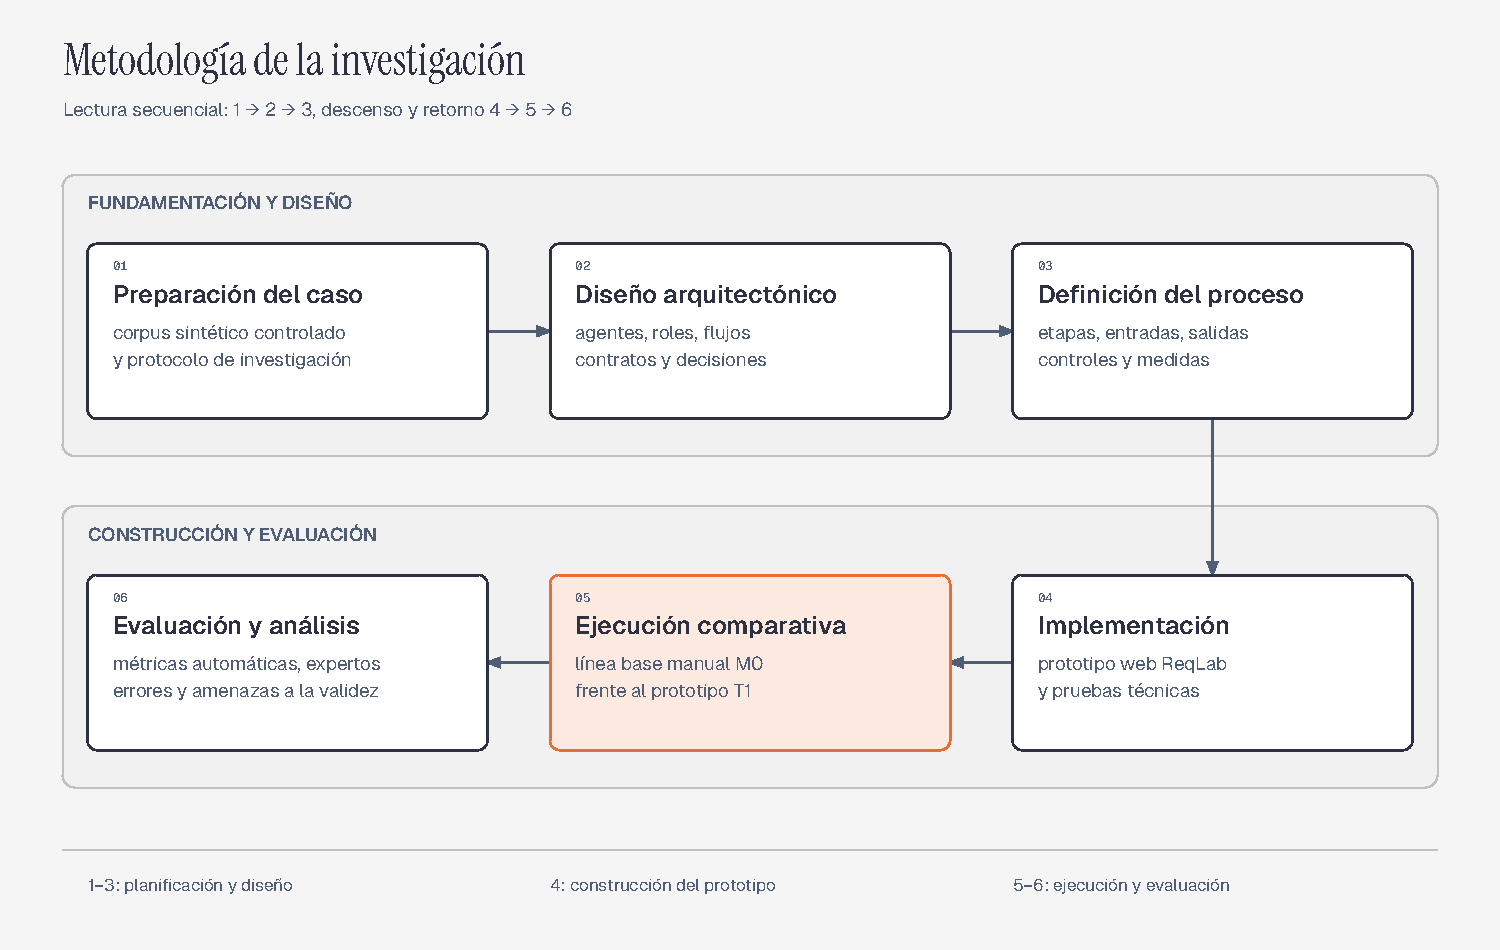
\includegraphics[width=\linewidth,height=0.90\textheight,keepaspectratio]{metodologia_integral.pdf}
  \caption{Fases metodológicas y relación entre diseño, implementación y evaluación.}
  \label{fig:metodologia}
\end{figure}
\end{landscape}

% !TEX root = ../main.tex
\chapter{Diseño de la arquitectura multiagente}
\label{cap:arquitectura}

\section{Propósito y alcance}

La arquitectura de ReqLab tiene como propósito transformar fuentes textuales no estructuradas en propuestas de RF, RNF e historias de usuario con evidencia verificable. Se adopta una coordinación centralizada y secuencial. Los agentes son unidades lógicas especializadas por responsabilidad, instrucciones, herramientas y contratos; no se afirma que posean autonomía general ni negociación libre.

El diseño se documenta mediante elementos adaptados de ISO/IEC/IEEE 42010:2022 \cite{iso42010}: interesados y preocupaciones, contexto, vistas, relaciones, decisiones y correspondencias. La norma orienta la descripción, sin declarar certificación ni conformidad formal.

\section{Interesados y preocupaciones}

\begin{table}[H]
  \centering
  \caption{Interesados y preocupaciones arquitectónicas}
  \label{tab:interesados-arquitectura}
  \small
  \begin{tabularx}{\textwidth}{p{3.4cm}YY}
    \toprule
    Interesado & Preocupación & Respuesta del diseño \\
    \midrule
    Usuario o analista & Trabajar por proyectos, aportar fuentes reales, aclarar decisiones y revisar salidas. & Interfaz web por etapas, vista previa, definición adaptativa, revisión y exportación. \\
    Experto evaluador & Inspeccionar evidencia y comparar productos de manera consistente. & Esquemas comunes, citas por fragmento, relaciones y reportes de validación. \\
    Investigador & Reproducir una corrida y explicar las condiciones utilizadas. & Huellas de fuentes, versiones, parámetros, telemetría y registros de ejecución. \\
    Tutora y tribunal & Verificar correspondencia entre objetivos, diseño e implementación. & Vistas arquitectónicas, contratos, decisiones y matriz de verificación. \\
    Desarrollador & Mantener el núcleo independiente del dominio y sustituir componentes. & Capas separadas, configuración externa e interfaces para LLM, recuperación y persistencia. \\
    \bottomrule
  \end{tabularx}
\end{table}

\section{Contexto y límites}

ReqLab es una aplicación web local de un solo usuario. Recibe archivos PDF, DOCX, TXT o Markdown y texto pegado; conserva los originales; extrae y segmenta su contenido; conduce una definición interactiva; genera artefactos; y permite revisarlos y exportarlos. El servicio LLM externo se utiliza en las tareas semánticas. Los embeddings, la recuperación, la persistencia y los controles deterministas se ejecutan localmente.

Quedan fuera del límite actual: OCR, transcripción automática de audio, autenticación, edición colaborativa multiusuario, aprobación automática de requisitos, resolución autónoma de conflictos, entrenamiento de modelos y comparación exhaustiva de arquitecturas o LLM. DeepSeek es el proveedor validado; otros servicios con interfaz semejante pueden requerir adaptación y no se consideran verificados por defecto.

\section{Vista de capas y componentes}

\begin{figure}[H]
  \centering
  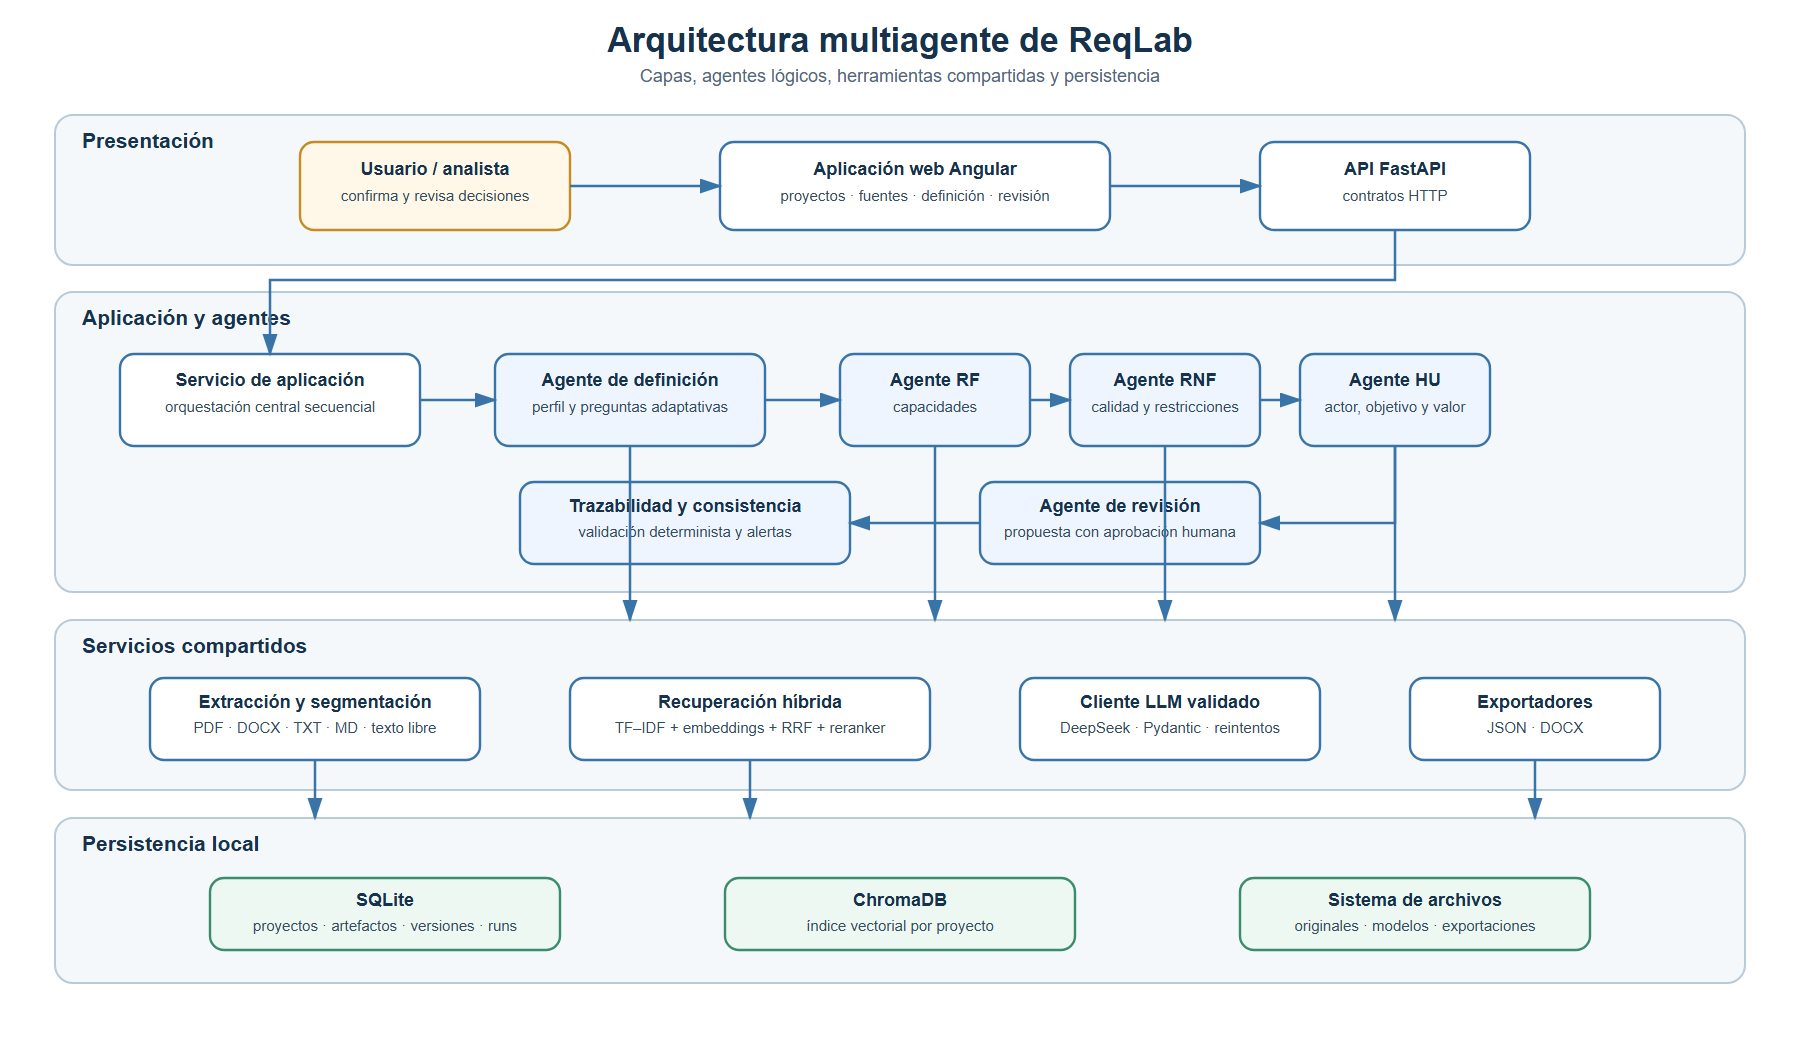
\includegraphics[width=\textwidth]{arquitectura_componentes.png}
  \caption{Vista de capas, componentes y agentes de ReqLab.}
  \label{fig:arquitectura-componentes}
\end{figure}

\begin{table}[H]
  \centering
  \caption{Responsabilidades de los componentes principales}
  \label{tab:componentes}
  \small
  \begin{tabularx}{\textwidth}{p{3.7cm}p{4.1cm}Y}
    \toprule
    Componente & Responsabilidad & Resultado \\
    \midrule
    Interfaz Angular & Gestionar proyectos y etapas de fuentes, definición, generación y revisión. & Acciones del usuario y visualización de evidencia. \\
    API FastAPI & Exponer casos de uso y validar solicitudes HTTP. & Contratos de entrada y respuesta. \\
    Servicio de aplicación & Coordinar transacciones, agentes, progreso, errores y persistencia. & Flujo reproducible por proyecto. \\
    Extracción y segmentación & Convertir fuentes y producir unidades citables según su tipo. & Catálogo de fragmentos. \\
    Agente de definición & Interpretar todo el corpus por lotes, construir perfil y formular aclaraciones. & Perfil provisional, preguntas y decisiones confirmadas. \\
    Recuperador híbrido & Combinar TF--IDF, embeddings y RRF; aplicar reranking opcional. & Evidencia ordenada por consulta especializada. \\
    Agentes RF, RNF y HU & Generar cada tipo conforme a su contrato y contexto previo. & Artefactos estructurados con citas y relaciones. \\
    Agente de trazabilidad y consistencia & Comprobar citas, relaciones, estructura, duplicados y clasificación. & Reporte y alertas por artefacto. \\
    Agente de revisión & Proponer una versión sustentada sin sobrescribir la vigente. & Propuesta aceptable o rechazable por el usuario. \\
    Persistencia & Guardar estado relacional, originales, vectores y exportaciones. & Historial auditable del proyecto. \\
    \bottomrule
  \end{tabularx}
\end{table}

\section{Agentes, roles y herramientas}

\begin{longtable}{p{3.0cm}p{4.0cm}p{3.8cm}p{3.0cm}}
  \caption{Agentes lógicos de la arquitectura}
  \label{tab:agentes-arquitectura}\\
  \toprule
  Agente & Entrada principal & Herramientas o reglas & Salida \\
  \midrule
  \endfirsthead
  \toprule
  Agente & Entrada principal & Herramientas o reglas & Salida \\
  \midrule
  \endhead
  Definición & Metadatos y todos los fragmentos documentales. & Análisis jerárquico por lotes, síntesis y esquema tipado. & Perfil provisional y preguntas trazables. \\
  Generación RF & Perfil confirmado y evidencia recuperada. & Consulta funcional, contrato RF y LLM. & Capacidades observables. \\
  Generación RNF & Perfil, evidencia y RF existentes. & Consulta de calidad, contrato RNF y LLM. & Restricciones y atributos verificables. \\
  Generación HU & Perfil, evidencia y artefactos existentes. & Consulta de actores/valor, contrato HU y LLM. & Historias y criterios de aceptación. \\
  Trazabilidad y consistencia & Artefactos y catálogo de fragmentos. & Reglas deterministas y umbrales configurables. & Validación, duplicados y relaciones inválidas. \\
  Revisión & Artefacto vigente, instrucción y evidencia recuperada. & Contrato de revisión y LLM. & Propuesta de nueva versión. \\
  \bottomrule
\end{longtable}

El recuperador y el servicio de extracción son herramientas compartidas, no agentes generativos adicionales. Esta delimitación evita inflar artificialmente el número de agentes y permite asociar cada intervención del LLM con un rol observable.

\section{Vista de interacción}

La interacción principal sigue una secuencia controlada:

\begin{enumerate}
  \item el usuario crea un proyecto y agrega fuentes por archivo o texto;
  \item el servicio extrae, segmenta, persiste e indexa incrementalmente los fragmentos;
  \item el agente de definición analiza el corpus completo mediante lotes y síntesis;
  \item el usuario corrige el perfil, responde preguntas y confirma la definición;
  \item las respuestas se convierten en fragmentos \codigo{USR-DEF-*} y se indexan;
  \item el orquestador ejecuta secuencialmente los agentes RF, RNF y HU;
  \item cada agente consulta al recuperador híbrido y recibe los artefactos previos como contexto generado;
  \item los esquemas tipados validan cada respuesta antes de persistirla;
  \item el agente de trazabilidad y consistencia crea alertas y validación por artefacto;
  \item el usuario inspecciona fuentes, edita manualmente o solicita una propuesta de revisión; y
  \item el proyecto se exporta a JSON o DOCX junto con su información de trazabilidad.
\end{enumerate}

Una fuente duplicada se detecta mediante su huella; una extracción vacía, esquema inválido o error de proveedor se informa explícitamente. Las alertas de contenido no se resuelven silenciosamente y una propuesta de revisión no sustituye al artefacto hasta que el usuario la acepte.

\section{Vista de información y trazabilidad}

\begin{figure}[H]
  \centering
  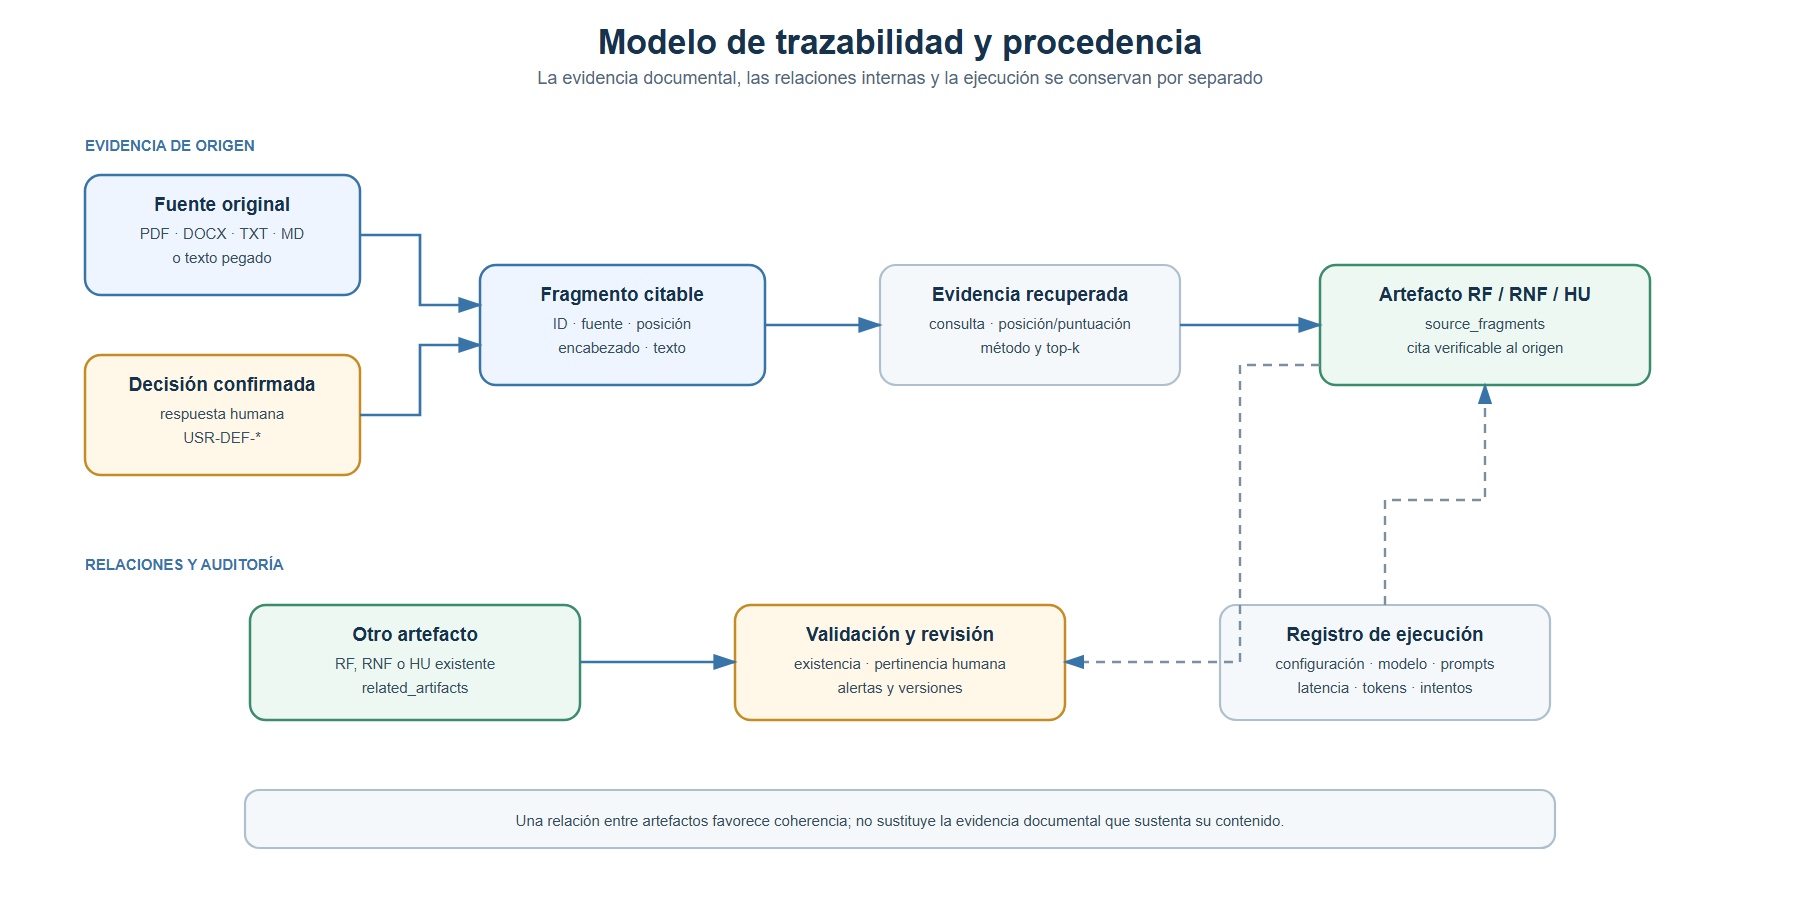
\includegraphics[width=\textwidth]{trazabilidad_informacion.png}
  \caption{Procedencia documental, relaciones entre artefactos y registro de ejecución.}
  \label{fig:arquitectura-informacion}
\end{figure}

La procedencia comienza en una fuente original o en una respuesta de definición confirmada. La segmentación produce un fragmento estable; la recuperación registra su posición o puntuación; y el artefacto conserva el identificador en \codigo{source_fragments}. De forma separada, \codigo{related_artifacts} relaciona RF, RNF y HU. La ejecución almacena la configuración y telemetría necesarias para interpretar cómo se obtuvo la salida.

\section{Contratos de información}

\begin{longtable}{p{3.1cm}p{5.5cm}p{5.8cm}}
  \caption{Contratos mínimos entre componentes}
  \label{tab:contratos-arquitectura}\\
  \toprule
  Objeto & Campos mínimos & Restricción \\
  \midrule
  \endfirsthead
  \toprule
  Objeto & Campos mínimos & Restricción \\
  \midrule
  \endhead
  Project & id, name, description, domain, status, definition\_confirmed & El contexto pertenece a un único proyecto. \\
  Source & source\_code, original\_name, source\_kind, hash, status & La huella no se repite dentro del proyecto. \\
  Fragment & fragment\_id, source\_id, source\_file, heading, text, position & El ID es único y conserva procedencia. \\
  Definition profile & dimensiones, valores, evidencia, confianza y confirmación & Las contradicciones no se resuelven sin respuesta del usuario. \\
  Retrieved evidence & fragment\_id, posición o puntuación, consulta y método & El fragmento debe existir en el catálogo. \\
  Artifact & artifact\_id, type, title, description, priority, source\_fragments, status, acceptance\_criteria, related\_artifacts & Tipo, prioridad, estado, citas y relaciones se validan contra el contexto permitido. \\
  Validation report & incidencias, duplicados, relaciones inválidas, umbrales y evaluación por artefacto & Informa; no aprueba ni corrige automáticamente. \\
  Run & fase, agente, estado, parámetros, métricas, inicio y fin & Conserva una instantánea de la configuración utilizada. \\
  \bottomrule
\end{longtable}

\section{Persistencia}

La persistencia se distribuye de acuerdo con la naturaleza de la información:

\begin{itemize}
  \item SQLite conserva proyectos, fuentes, fragmentos, preguntas, perfiles, artefactos, versiones, propuestas, validaciones y ejecuciones;
  \item ChromaDB conserva los embeddings y el índice semántico separado por proyecto y versión de modelo; y
  \item el sistema de archivos conserva documentos originales, caché local de modelos y exportaciones.
\end{itemize}

Esta combinación no introduce lógica de dominio. SQLite proporciona integridad transaccional e historial; ChromaDB permite recuperación vectorial; y los originales permanecen disponibles para vista previa y auditoría.

\section{Decisiones arquitectónicas}

\begin{table}[H]
  \centering
  \caption{Decisiones y justificación}
  \label{tab:decisiones-arquitectura}
  \small
  \begin{tabularx}{\textwidth}{p{3.7cm}YY}
    \toprule
    Decisión & Justificación & Consecuencia o límite \\
    \midrule
    Orquestación central secuencial & Facilita auditoría, control de estados y correspondencia con el proceso. & Menor autonomía y paralelismo. \\
    Agentes lógicos especializados & Separa definición, RF, RNF, HU, control y revisión. & La especialización no demuestra por sí sola mayor calidad. \\
    Definición antes de generar & Incorpora decisiones humanas que el corpus no permite inferir. & Añade una interacción obligatoria cuando existen vacíos relevantes. \\
    Recuperación híbrida & Combina coincidencia terminológica y proximidad semántica. & Requiere modelos locales y parámetros que deben registrarse. \\
    Reranker opcional & Permite una segunda evaluación de relevancia sin volverla requisito del MVP. & Aumenta latencia y debe evaluarse antes de atribuir beneficio. \\
    Esquemas tipados y reintentos & Impiden persistir respuestas que violen contratos conocidos. & No garantizan corrección semántica. \\
    Evidencia separada de relaciones & Evita tratar artefactos generados como fuentes documentales. & Requiere dos tipos de enlace explícitos. \\
    Revisión con aprobación humana & Conserva control sobre cambios y versiones. & El flujo no es completamente autónomo. \\
    Aplicación web y Docker & Facilitan demostración y repetición del entorno. & El MVP sigue siendo local y monousuario. \\
    \bottomrule
  \end{tabularx}
\end{table}

\section{Correspondencia entre diseño e implementación}

\begin{table}[H]
  \centering
  \caption{Correspondencia de arquitectura, código y verificación}
  \label{tab:correspondencia-codigo}
  \small
  \begin{tabularx}{\textwidth}{p{3.5cm}p{5.1cm}Y}
    \toprule
    Elemento & Implementación & Verificación \\
    \midrule
    Interfaz y API & \codigo{frontend/src/app} y \codigo{api/routers}. & Compilación Angular y pruebas de flujo HTTP. \\
    Extracción & \codigo{documents.py}. & Formatos, fuente libre y segmentación por tipo. \\
    Definición & \codigo{agents.py} y \codigo{services.py}. & Cobertura del corpus, preguntas dinámicas y confirmación. \\
    Recuperación híbrida & \codigo{retrieval.py} y \codigo{vector_store.py}. & Prefijos, fusión, top--k, reranker e indexación incremental. \\
    Generación especializada & Contratos de \codigo{agents.py}. & RF/RNF/HU, citas, relaciones y esquemas tipados. \\
    Control y revisión & \codigo{validation.py} y \codigo{RevisionAgent}. & Incidencias, umbrales, propuesta, aceptación y versión. \\
    Persistencia y exportación & \codigo{storage.py} y \codigo{exporters.py}. & Integridad, configuración de corrida y archivos JSON/DOCX. \\
    \bottomrule
  \end{tabularx}
\end{table}

\section{Verificación del objetivo específico 1}

El objetivo se verifica mediante una lista de comprobación que confirme interesados, propósito y límites; capas y componentes; agentes y responsabilidades; secuencia e interacción; contratos y flujos de información; persistencia; trazabilidad entre vistas; decisiones y consecuencias; y correspondencia con código y pruebas.

El criterio del proyecto exige que todos los elementos aplicables estén documentados y que no existan contradicciones sin justificar entre las vistas. ISO/IEC/IEEE 42010 no impone un porcentaje universal. Con la especificación actual existe evidencia de diseño para el objetivo 1, sujeta a revisión académica y a mantener sincronizada la correspondencia cuando el prototipo cambie.

% !TEX root = ../main.tex
\chapter{Proceso de transformación de fuentes textuales}
\label{cap:proceso}

\section{Propósito y alcance}

Este capítulo define cómo ReqLab transforma fuentes textuales no estructuradas en RF, RNF e historias de usuario. Especifica entradas, operaciones, salidas, controles y medidas para las seis etapas nombradas en el objetivo específico 2: segmentación, recuperación contextual, generación, trazabilidad, validación y verificación de consistencia. La ingesta y definición preparan la entrada; la revisión y exportación controlan la salida. Por tanto, estas actividades amplían la operación del prototipo sin modificar el objetivo aprobado.

La estructura se apoya en ISO/IEC/IEEE 29148:2018 para la especificación, trazabilidad y verificación de requisitos \cite{iso29148}, y en ISO/IEC/IEEE 15939:2017 para definir medidas \cite{iso15939}. La adaptación no constituye certificación.

\section{Condiciones de entrada}

Una ejecución parte de un proyecto con nombre, descripción y dominio. El usuario carga PDF con texto seleccionable, DOCX, TXT o Markdown, o pega directamente un correo, entrevista, conversación, nota u otro texto. No se exige una estructura interna ni identificadores previos. Cada fuente conserva nombre, tipo declarado, huella SHA--256, estado y archivo original cuando corresponda.

El proceso automatiza extracción, segmentación, recuperación, generación y controles. No aprueba requisitos ni elige por sí mismo entre reglas contradictorias. Los artefactos resultantes son propuestas revisables.

\section{Flujo general}

\begin{figure}[H]
  \centering
  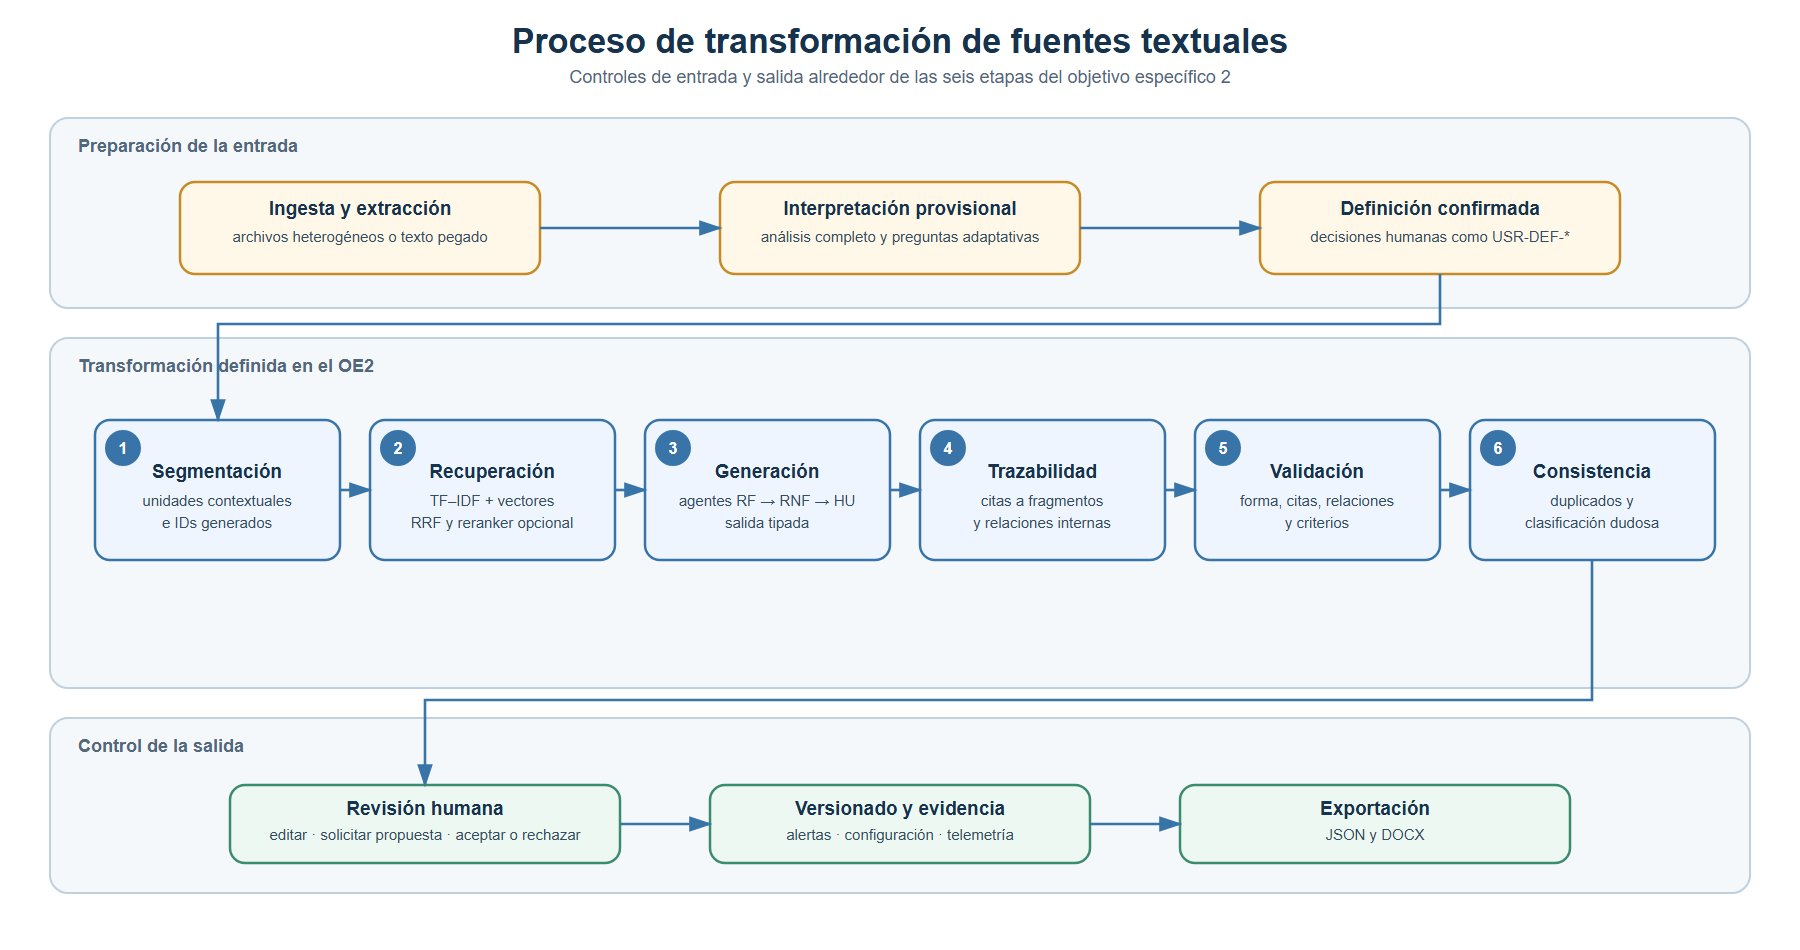
\includegraphics[width=\textwidth]{proceso_transformacion.png}
  \caption{Flujo operativo de transformación y controles de entrada y salida.}
  \label{fig:proceso-transformacion}
\end{figure}

\section{Controles previos}

\subsection{Ingesta y extracción}

La extracción convierte el contenedor en texto y rechaza formatos no admitidos, fuentes duplicadas o contenido no utilizable. La vista previa permite al usuario verificar el contenido interpretado y eliminar una fuente. Cualquier cambio invalida la definición y los resultados dependientes, evitando conservar artefactos como si provinieran del corpus vigente.

\subsection{Definición interactiva}

El agente de definición recorre todos los fragmentos documentales mediante análisis por lotes y una síntesis global. Produce un perfil provisional con evidencia y niveles de confianza, y formula preguntas solo para ausencias, baja confianza, contradicciones o decisiones que cambian el sistema. El usuario revisa el perfil y responde las aclaraciones obligatorias. Al confirmar, sus respuestas se persisten e indexan como fragmentos \codigo{USR-DEF-*}.

La salida de este control es una interpretación confirmada que se entrega a los agentes de generación. Si cambian las fuentes, debe repetirse la definición. Esta regla evita utilizar respuestas pertenecientes a una versión anterior del corpus.

\section{Etapas del objetivo específico 2}

\subsection{Etapa 1: segmentación}

\textbf{Objetivo.} Convertir el texto extraído en unidades recuperables y citables.

\textbf{Entrada.} Texto de la fuente, código, nombre y tipo declarado.

\textbf{Operación.} El segmentador identifica unidades naturales según el tipo: encabezados de correo, turnos de entrevista o conversación, secciones Markdown o párrafos. Las unidades extensas se dividen por tamaño con solapamiento.

\textbf{Parámetros iniciales.} Tamaño máximo de 1,200 caracteres y solapamiento de 180. Son valores configurables que se congelarán antes del experimento.

\textbf{Salida.} Fragmentos con ID generado, fuente, encabezado, posición y texto.

\textbf{Control.} Debe existir al menos un fragmento utilizable y sus IDs deben ser únicos dentro del proyecto.

\subsection{Etapa 2: recuperación contextual}

\textbf{Objetivo.} Seleccionar evidencia pertinente para cada agente sin depender del orden de carga ni enviar indiscriminadamente todo el corpus.

\textbf{Entrada.} Fragmentos documentales y de definición, metadatos del proyecto y consulta especializada del agente.

\textbf{Operación.} Se ejecutan recuperación TF--IDF y búsqueda semántica mediante embeddings. Las posiciones se combinan con RRF usando pesos configurables; opcionalmente, un \emph{cross-encoder} reordena los candidatos.

\textbf{Parámetros candidatos después de la calibración técnica.} \(w_l=0.45\), \(w_s=0.55\), \(top\_k=12\), embeddings \codigo{intfloat/multilingual-e5-base} y reranker desactivado. E5 Base se seleccionó por su orientación a recuperación multilingüe y una longitud de entrada compatible con los fragmentos del proyecto. El reranker MMARCO permanece implementado como opción configurable, pero la comparación inicial no mostró una mejora consistente de cobertura frente a la latencia añadida. La configuración utilizada definitivamente se congelará y almacenará en la ejecución experimental.

\textbf{Salida.} Lista ordenada de IDs, puntuaciones o posiciones y texto suministrado al agente.

\textbf{Control.} Los IDs recuperados deben pertenecer al proyecto; la colección vectorial se versiona por modelo y prefijos.

\subsection{Etapa 3: generación estructurada}

\textbf{Objetivo.} Producir propuestas de RF, RNF y HU respaldadas por evidencia.

\textbf{Entrada.} Definición confirmada, evidencia recuperada, contrato tipado, reglas del \emph{prompt} y artefactos generados previamente.

\textbf{Operación.} El orquestador invoca agentes especializados en el orden RF--RNF--HU. Cada agente dispone de una tarea y consulta propia. Los artefactos ya generados se utilizan como contexto de coherencia, pero nunca como citas documentales.

\textbf{Configuración inicial.} Proveedor DeepSeek, modelo \codigo{deepseek-chat}, temperatura (0.1) y hasta tres intentos de validación. Antes de iniciar, el sistema calcula con \codigo{evidence-budget-v1} un intervalo independiente para RF, RNF y HU según las unidades de evidencia y los indicios generales de cada tipo. La interfaz precarga el valor sugerido y permite al usuario seleccionar un máximo dentro del intervalo. El valor se expresa como ``hasta \(n\)'': no obliga a completar una cuota y el agente debe devolver menos artefactos si carece de sustento.

\textbf{Salida.} Objetos tipados con identificador, tipo, título, descripción, prioridad, estado, citas, criterios de aceptación y relaciones.

\textbf{Control.} La respuesta debe satisfacer el esquema Pydantic y citar únicamente fragmentos permitidos. El \emph{prompt} enumera los identificadores de evidencia y relación admitidos mediante ejemplos construidos con datos reales de la recuperación, no con marcadores descriptivos. Si la respuesta supera el presupuesto, el exceso se descarta de forma determinista y el evento queda registrado, sin consumir reintentos para corregir solamente la cantidad. El método, sus entradas, la recomendación y la selección quedan almacenados. Agotados los intentos por JSON inválido o incumplimiento del contrato, la etapa falla de forma explícita y conserva el motivo específico del último rechazo.

\subsection{Etapa 4: construcción de trazabilidad}

\textbf{Objetivo.} Hacer inspeccionable la procedencia y la correspondencia interna.

\textbf{Operación.} \codigo{source_fragments} enlaza el artefacto con documentos o decisiones confirmadas; \codigo{related_artifacts} enlaza RF, RNF y HU. Ambos espacios se validan por separado.

\textbf{Regla mínima.} Todo artefacto debe declarar al menos un fragmento existente. Una relación interna debe apuntar a otro artefacto del mismo proyecto. La existencia no prueba pertinencia semántica.

\textbf{Salida.} Evidencia visible por artefacto y relaciones navegables en revisión y exportación.

\subsection{Etapa 5: validación estructural}

\textbf{Objetivo.} Comprobar los contratos antes de la evaluación experta.

\textbf{Operación.} Se identifican citas o relaciones ausentes e inexistentes, valores no permitidos, descripciones incompletas, HU sin estructura mínima y HU sin criterios de aceptación. Parte de estas restricciones se aplica al recibir la salida del LLM y parte se consolida en el reporte del proyecto.

\textbf{Salida.} Resultado general y observaciones asociadas con cada artefacto. El informe no lo modifica automáticamente.

\subsection{Etapa 6: verificación de consistencia}

\textbf{Objetivo.} Señalar indicios de redundancia o clasificación inconsistente para revisión humana.

\textbf{Operación.} Se calcula similitud de Jaccard entre artefactos del mismo tipo y, con un umbral separado, entre tipos distintos. También se aplican reglas conservadoras para detectar RNF con redacción funcional.

\textbf{Parámetros iniciales.} Umbral de 0.72 para duplicados del mismo tipo y 0.55 para duplicados cruzados. Son heurísticas configurables y no reglas universales de calidad.

\textbf{Salida.} Pares candidatos, puntuación, motivo y observaciones. Ninguna alerta fusiona, reclasifica o descarta un artefacto.

\section{Control posterior: revisión y exportación}

El usuario puede editar manualmente un artefacto, cambiar su clasificación o describir qué desea mejorar. En el segundo caso, el agente de revisión recupera evidencia y crea una propuesta separada. La versión vigente solo cambia si el usuario acepta; el rechazo también queda registrado. Las observaciones automáticas enlazan los elementos afectados con estas acciones, pero nunca realizan correcciones autónomas. Cada modificación genera una versión y actualiza la validación. Una reclasificación asigna un identificador coherente con el nuevo tipo y actualiza de forma versionada las relaciones que utilizaban el identificador anterior.

La exportación produce JSON para análisis y DOCX para lectura o entrega. Ambos formatos incluyen artefactos y procedencia; el reporte técnico incorpora la configuración de la ejecución cuando está disponible.

\section{Tratamiento de incidencias}

\begin{table}[H]
  \centering
  \caption{Reglas de tratamiento de incidencias}
  \label{tab:incidencias-proceso}
  \small
  \begin{tabularx}{\textwidth}{p{4.1cm}YY}
    \toprule
    Situación & Respuesta automática & Acción posterior \\
    \midrule
    Formato no admitido, extracción vacía o fuente duplicada & Rechazar la fuente e informar la causa. & Convertir, corregir o seleccionar otra fuente. \\
    Cambio de fuente tras definición & Invalidar perfil confirmado y resultados dependientes. & Repetir análisis y confirmación. \\
    Esquema LLM inválido & Reintentar con el error de validación hasta el máximo. & Corregir configuración o revisar proveedor si falla. \\
    Cita o relación inválida & Rechazar durante validación tipada o registrar incidencia. & Regenerar o editar con evidencia válida. \\
    Posible duplicado o clasificación dudosa & Emitir alerta sin modificar. & Revisar y decidir consolidación o clase. \\
    Cambio de modelo vectorial & Usar una colección versionada compatible. & Reindexar en el nuevo espacio. \\
    Error de proveedor & Finalizar la ejecución como fallida y conservar el mensaje. & Reintentar cuando el servicio esté disponible. \\
    \bottomrule
  \end{tabularx}
\end{table}

\section{Registros de evidencia}

\begin{table}[H]
  \centering
  \caption{Evidencia conservada por ReqLab}
  \label{tab:salidas-corrida}
  \small
  \begin{tabularx}{\textwidth}{p{4.0cm}Y}
    \toprule
    Registro & Contenido \\
    \midrule
    Proyecto y fuentes & Metadatos, originales, tipo, huella, estado y fragmentos. \\
    Definición & Perfil provisional, evidencia, preguntas, respuestas y confirmación. \\
    Artefactos y versiones & RF, RNF, HU, citas, relaciones, cambios y origen de revisión. \\
    Validación & Incidencias, duplicados, umbrales y observaciones por artefacto. \\
    Ejecuciones & Fase, agente, estado, configuración, latencia, tokens, intentos y errores. \\
    Exportaciones & Representación JSON o documento DOCX descargable. \\
    \bottomrule
  \end{tabularx}
\end{table}

\section{Medidas de verificación}

\begin{longtable}{p{4.0cm}p{5.8cm}p{4.8cm}}
  \caption{Medidas definidas para verificar el proceso}
  \label{tab:medidas-proceso}\\
  \toprule
  Necesidad & Medida & Criterio del proyecto \\
  \midrule
  \endfirsthead
  \toprule
  Necesidad & Medida & Criterio del proyecto \\
  \midrule
  \endhead
  Especificación del proceso & Etapas del OE2 con entrada, operación, salida y control / 6 \(\times 100\) & Debe documentarse el 100\,\% de las etapas. \\
  Cobertura del análisis de definición & Fragmentos documentales analizados / fragmentos disponibles \(\times 100\) & Meta de 100\,\% según el registro de cobertura. \\
  Cobertura de trazabilidad & Artefactos con al menos una cita válida / total \(\times 100\) & Meta operativa de 100\,\% antes de evaluación. \\
  Integridad de citas & Artefactos con cita inválida / total \(\times 100\) & Meta de 0\,\%; cualquier caso requiere revisión. \\
  Integridad de relaciones & Relaciones inexistentes / relaciones declaradas \(\times 100\) & Meta de 0\,\%. \\
  Conformidad de HU & HU sin error de forma ni criterios / total de HU \(\times 100\) & Meta operativa de 100\,\%. \\
  Reproducibilidad & Campos de configuración presentes / campos requeridos \(\times 100\) & Meta de 100\,\% en la corrida experimental. \\
  \bottomrule
\end{longtable}

Los porcentajes son criterios de aceptación de esta investigación. Las normas orientan cómo definir y comunicar medidas, pero no establecen esos umbrales de forma universal.

\section{Verificación del objetivo específico 2}

El objetivo 2 se considera documentado cuando sus seis etapas disponen de propósito, entrada, operación, salida, control y tratamiento de errores; la definición previa y revisión posterior tienen límites claros; los contratos permiten seguir la procedencia; y las medidas pueden calcularse a partir de los registros. La especificación actual cubre esos elementos. Los valores obtenidos y hallazgos se incorporarán después de congelar y ejecutar el experimento.

% !TEX root = ../main.tex
\chapter{Implementación del prototipo}
\label{cap:implementacion}

\section{Estado y alcance de la implementación}

ReqLab implementa una aplicación web para organizar múltiples proyectos, incorporar fuentes heterogéneas, definir interactivamente el sistema, generar RF, RNF e historias de usuario, revisar la evidencia y exportar resultados. El núcleo no contiene actores ni reglas de SIGSAT u otro caso específico: cada proyecto se interpreta desde sus propias fuentes y respuestas.

La versión documentada de la API es 0.3.0. El prototipo se encuentra en estado funcional para desarrollo y demostración. No obstante, el cierre académico del objetivo específico 3 requiere ejecutar la matriz formal de aceptación y conservar una corrida integral con la configuración congelada.

\section{Tecnologías y despliegue}

\begin{table}[H]
  \centering
  \caption{Tecnologías principales del prototipo}
  \label{tab:tecnologias-prototipo}
  \small
  \begin{tabularx}{\textwidth}{p{3.5cm}p{4.0cm}Y}
    \toprule
    Capa & Tecnología & Función \\
    \midrule
    Presentación & Angular y TypeScript & Interfaz por proyectos y etapas reutilizables. \\
    API & FastAPI y Pydantic & Servicios HTTP, validación de solicitudes y contratos tipados. \\
    Aplicación & Python & Orquestación, agentes, extracción, recuperación y validación. \\
    Persistencia relacional & SQLite & Estado, preguntas, artefactos, versiones, ejecuciones y reportes. \\
    Persistencia vectorial & ChromaDB & Embeddings e índice semántico aislado por proyecto. \\
    Procesamiento semántico local & sentence-transformers & Embeddings locales y reranking opcional. \\
    Servicios semánticos externos & DeepSeek y Jev vía OpenRouter & Interpretación, generación, revisión y opciones de reranking o validación semántica. \\
    Documentos & pypdf y python-docx & Extracción de PDF/DOCX y exportación DOCX. \\
    Despliegue & Docker Compose y Nginx & Contenedores de API e interfaz con volumen persistente. \\
    \bottomrule
  \end{tabularx}
\end{table}

La clave del proveedor se lee desde variables de entorno y no se incorpora al repositorio ni al documento de tesis. Docker Compose expone la interfaz y la API, y monta el directorio de datos para conservar proyectos entre reinicios.

\section{Organización del código}

\begin{table}[H]
  \centering
  \caption{Módulos del prototipo}
  \label{tab:modulos-prototipo}
  \small
  \begin{tabularx}{\textwidth}{p{4.8cm}p{3.5cm}Y}
    \toprule
    Módulo & Elemento principal & Responsabilidad \\
    \midrule
    Frontend Angular & Componentes, rutas y estado & Proyectos, fuentes, definición, generación y revisión. \\
    \codigo{api/routers} & Rutas FastAPI & Contratos HTTP por recurso y caso de uso. \\
    \codigo{services.py} & Servicio de aplicación & Coordinación transaccional del flujo. \\
    \codigo{documents.py} & Extracción y segmentación & PDF, DOCX, TXT, Markdown y texto pegado. \\
    \codigo{vector_store.py} & Repositorio y recuperador híbrido & Índice, embeddings, RRF y reranking. \\
    \codigo{retrieval.py} & TfidfRetrievalAgent & Recuperación léxica local. \\
    \codigo{jev\_reranker.py} & JevReranker & Reordenamiento remoto opcional y auditoría de candidatos. \\
    \codigo{agents.py} & Agentes y contratos & Definición, RF, RNF, HU y revisión. \\
    \codigo{llm.py} y \codigo{llm_schemas.py} & Cliente y esquemas Pydantic & Invocación, validación, reintentos y telemetría. \\
    \codigo{validation.py} & Validador de trazabilidad & Citas, relaciones, estructura y duplicados. \\
    \codigo{semantic\_validation.py} y \codigo{typesafe\_client.py} & Piloto Jev & Evaluación semántica en modo \emph{shadow} y cliente remoto desacoplado. \\
    \codigo{storage.py} & SQLiteRepository & Persistencia, migraciones e historial. \\
    \codigo{exporters.py} & Exportadores & Salidas JSON y DOCX. \\
    \bottomrule
  \end{tabularx}
\end{table}

\section{Gestión de proyectos y fuentes}

La pantalla inicial permite crear, listar, archivar, desarchivar y eliminar proyectos. El archivado es reversible y no elimina sus datos. Cada proyecto mantiene un estado coherente con el flujo, y se impiden operaciones destructivas mientras la generación está en curso.

Las fuentes pueden cargarse como archivos o registrarse pegando texto con un título y tipo. La extracción admite PDF textual, DOCX, TXT y Markdown. El sistema calcula una huella SHA--256 para evitar duplicados, conserva el original, genera un código de fuente y permite previsualizar o eliminar el documento. Al eliminarlo también se retiran sus vectores y se invalidan la definición y resultados dependientes.

\section{Segmentación e indexación incremental}

\codigo{TextSegmentationService} recibe \codigo{source_kind} y aplica reglas acordes al contenido: correo, entrevista, conversación, notas o documento general. Si una unidad natural excede el tamaño máximo, utiliza ventanas con solapamiento. Cada fragmento conserva un ID generado y la referencia a su fuente.

\codigo{ChromaProjectVectorStore} calcula embeddings locales y realiza \emph{upsert} o eliminación selectiva. De esta forma, una nueva fuente no obliga a recalcular todo el proyecto. La colección incluye una huella del modelo y de los prefijos de consulta/pasaje; si cambia el espacio vectorial se utiliza una colección compatible y se evita mezclar dimensiones.

\section{Etapa de definición}

\codigo{ProjectDefinitionAgent} evita asumir que la información importante se encuentra en los primeros fragmentos. Divide el corpus completo en lotes configurables de 18\,000 caracteres y utiliza hasta tres trabajadores para analizarlos en paralelo. Cada lote completado se almacena como punto de control junto con una huella de su contenido. Después consolida localmente las coincidencias textuales por dimensión, reúne sus citas y conserva por separado las formulaciones distintas. Con esa entrada construye un perfil provisional y formula preguntas para dimensiones ausentes o de baja confianza, contradicciones y decisiones relevantes. Si falla la síntesis final, el siguiente intento reutiliza los lotes cuya huella no cambió y repite únicamente la operación pendiente.

El usuario puede revisar la interpretación antes de confirmar. Las respuestas obligatorias resueltas se almacenan en SQLite y se convierten en fragmentos \codigo{USR-DEF-*}, los cuales ingresan al índice. La API admite campos de definición extensos con un límite de seguridad de 20\,000 caracteres, de modo que una interpretación obtenida de un corpus amplio no sea rechazada al confirmarse. Si se modifica una fuente, la confirmación se invalida. Si se reconfirma una definición después de haber generado artefactos, Angular presenta una advertencia explícita: al aceptar, se eliminan los artefactos, versiones, observaciones y ejecuciones de generación anteriores, mientras se conservan fuentes y respuestas. El backend exige el indicador \codigo{reset\_generation} cuando detecta resultados existentes, por lo que esta regla no depende únicamente de la interfaz. Esta implementación conecta la elicitación humana con la generación sin presentar inferencias del LLM como hechos confirmados ni mezclar salidas de definiciones distintas.

\section{Recuperación híbrida}

\codigo{HybridRetrievalAgent} combina una lista léxica TF--IDF con una lista semántica obtenida desde ChromaDB. Los resultados se fusionan mediante RRF y pesos configurables. El soporte de prefijos distintos para consultas y pasajes permite utilizar correctamente familias de embeddings que requieren esa convención. Cuando el reranker está habilitado, la configuración del proyecto selecciona el \emph{cross-encoder} multilingüe local o Jev vía OpenRouter antes de limitar el contexto. La selección se conserva en SQLite y se incluye en la instantánea experimental.

El reranker Jev registra todos los candidatos considerados, su posición y puntuación RRF, las probabilidades de relevancia y evidencia útil, el promedio aplicado, la posición final y la selección. También conserva modelo solicitado y servido, proveedor, intentos, tokens, costo informado y latencia. Los errores 429 y 5xx se reintentan de forma acotada; si el servicio falla no se sustituye silenciosamente por el modelo local.

Cada contrato de generación define una consulta propia para favorecer evidencia funcional, atributos de calidad o actores y valor. El efecto de estas consultas deberá comprobarse en la evaluación; su contenido y el \(top\_k\) quedan registrados como condiciones de la ejecución.

\section{Generación multiagente}

El servicio ejecuta tres instancias de \codigo{SpecializedGenerationAgent} en secuencia: RF, RNF y HU. Cada una recibe un contrato con identificador, tarea, reglas y consulta de recuperación. Los artefactos consolidados en pasos anteriores se añaden como contexto para reducir aislamiento y favorecer relaciones, pero el \emph{prompt} prohíbe convertirlos en \codigo{source_fragments}. Al completar cada tipo, el servicio persiste sus artefactos, recuperación y telemetría como punto de control. Una ejecución interrumpida puede continuar desde el primer agente pendiente y reutiliza los límites y la configuración de la corrida original.

Antes de esa ejecución, \codigo{generation\_budget.py} recorre todos los fragmentos confirmados y calcula mínimos, sugerencias y máximos independientes. El endpoint \codigo{GET /generation/recommendations} expone el cálculo a Angular. La pantalla de generación muestra tres controles deslizantes ---RF, RNF y HU---, informa el volumen analizado y rotula cada selección como un máximo. \codigo{POST /generation} recibe los tres valores; el campo anterior \codigo{limit\_per\_type} se conserva para compatibilidad con clientes previos. El orquestador aplica el valor correspondiente a cada agente y almacena tanto la recomendación como la selección en los parámetros de la corrida. Al finalizar, la interfaz compara el máximo solicitado con la cantidad producida por tipo y explica que una cantidad inferior es válida cuando la evidencia o la validación impiden justificar más artefactos.

La respuesta se valida con modelos Pydantic. Se controlan tipo, prioridad, procedencia de prioridad, estado, criterios, citas y relaciones permitidas. El contrato añade patrón EARS y criterios de verificación para RF y RNF; para RNF incorpora categoría, métrica, unidad, umbral y método de verificación. Los campos no sustentados se conservan vacíos y el estado puede indicar que se requiere aclaración. Una prioridad sin procedencia explícita se transforma en \emph{No definida}, en lugar de asumir un nivel medio. El ejemplo JSON se construye con identificadores realmente autorizados para evitar que el LLM copie marcadores inválidos. Cuando la respuesta incumple el esquema, el cliente puede reintentar hasta el máximo configurado usando el error como retroalimentación. Si todos los intentos fallan, la telemetría y el mensaje de la corrida incluyen una síntesis segura del último error de validación. No existe una llamada posterior que omita la validación.

\section{Validación, revisión y exportación}

\codigo{TraceabilityConsistencyAgent} verifica citas y relaciones, conformidad EARS de RF, criterios de verificación, completitud de medición de RNF, procedencia de prioridad, conformidad de HU, indicios de clasificación y duplicación. Los posibles duplicados se separan entre pares del mismo tipo y pares cruzados. Cada observación se asocia con los artefactos correspondientes y la interfaz la presenta como alerta, no como corrección automática.

El usuario puede abrir cada observación y localizar directamente el artefacto implicado. Desde el panel de revisión puede modificar redacción, clasificación, prioridad, patrón EARS, criterios de verificación, campos de medición de RNF y criterios de aceptación, cambiar el estado o solicitar a \codigo{RevisionAgent} una propuesta sustentada. La propuesta se conserva aparte y puede aceptarse o rechazarse. Una reclasificación modifica el prefijo legible, actualiza referencias internas y crea versiones tanto para el artefacto como para las relaciones afectadas. Cada cambio recalcula la validación.

La revisión incluye aprobación masiva con advertencia previa y un gestor de prioridades para preparar varios cambios, aplicar un valor común a todos los artefactos y guardarlos de manera controlada. La prioridad sigue disponible en la edición individual. Las decisiones realizadas desde cualquiera de las dos vías se registran con procedencia humana.

El piloto opcional de validación semántica envía a Jev el artefacto y sus fragmentos citados, y almacena un informe independiente sobre respaldo conjunto y aporte de cada enlace. Funciona solo en modo \emph{shadow}: no cambia contenido, clasificación ni estado, y se marca como obsoleto cuando cambian el artefacto o sus citas.

Finalmente, el proyecto puede exportarse como JSON o DOCX. La salida documental presenta cada artefacto mediante una tabla de dos columnas adaptada a RF, RNF o HU e incluye una matriz de trazabilidad tabular con fragmento, fuente y extracto de evidencia.

\section{Observabilidad y reproducibilidad}

Cada agente y el orquestador registran inicio, fin, estado y error. Las llamadas al LLM capturan latencia, tokens reportados por el proveedor e intentos de validación. La ejecución principal agrega esas medidas y almacena una instantánea del modelo, embeddings, prefijos, proveedor y modelo de reranking, pesos de RRF, \(top\_k\), tamaño de fragmento, solapamiento, umbrales y versión de \emph{prompts}. La interfaz separa el consumo registrado para definición, generación, revisiones, validación semántica y Jev.

La telemetría permite auditar costos y comparar ejecuciones, pero no se interpreta como medida directa de calidad. Si el proveedor no informa tokens, el valor se registra como no disponible y no como cero.

\section{Pruebas implementadas}

El repositorio contiene 65 pruebas automatizadas. Estas pruebas no consumen proveedores externos; utilizan dobles controlados para comprobar contratos y flujo. Entre ellas se comprueba que una prioridad ausente no se convierta silenciosamente en media, que el validador detecte incumplimientos EARS, que la reanudación no repita agentes completados y que la auditoría de Jev conserve candidatos y telemetría. La ejecución completa, incluida la prueba de exportación que depende de \codigo{python-docx}, deberá repetirse sin omisiones en el entorno congelado y conservarse como evidencia de aceptación.

\begin{table}[H]
  \centering
  \caption{Cobertura actual de pruebas automatizadas}
  \label{tab:pruebas-prototipo}
  \small
  \begin{tabularx}{\textwidth}{p{5.2cm}Y}
    \toprule
    Área & Propiedades verificadas \\
    \midrule
    Proyectos y fuentes & Creación, archivo, eliminación, vista previa, duplicados e invalidación. \\
    Segmentación & Transmisión del tipo de fuente y conservación de unidades contextuales. \\
    Recuperación & Prefijos de consulta/pasaje, \(top\_k\), reranking local/Jev, auditoría de candidatos e índice incremental. \\
    Definición & Cobertura de todos los fragmentos por lotes, consolidación local, puntos de control, preguntas, respuestas y fragmentos confirmados. \\
    Generación & Orden de agentes, esquemas, presupuestos independientes, puntos de control, reanudación, diagnóstico de reintentos y relaciones. \\
    Telemetría & Latencia, intentos, consumo por fase y agregación sin duplicar ejecuciones reutilizadas. \\
    Validación y revisión & Citas, relaciones, duplicados, piloto semántico, reinicio explícito, edición, prioridad masiva, aprobación y versiones. \\
    Flujo web y exportación & Endpoints principales, navegación Angular y exportación tabular JSON/DOCX. \\
    \bottomrule
  \end{tabularx}
\end{table}

Además, la compilación de producción de Angular finaliza sin errores. Estas evidencias demuestran comportamiento técnico, pero no sustituyen la prueba de aceptación integral ni el juicio experto.

\section{Criterios pendientes para cerrar el objetivo específico 3}

Para considerar completado el objetivo 3 se deberá:

\begin{enumerate}
  \item congelar la versión de código y configuración;
  \item ejecutar el despliegue completo mediante Docker;
  \item aplicar la matriz de aceptación con el corpus SIGSAT-1.0;
  \item registrar entradas, resultados esperados, observados y evidencia;
  \item conservar una corrida real de definición, generación, revisión y exportación; y
  \item documentar limitaciones e incidentes observados.
\end{enumerate}

La implementación constituye un avance sustancial y coherente con la arquitectura actual; el cierre del objetivo depende de reunir esa evidencia formal.

% !TEX root = ../main.tex
\chapter{Evaluación experimental y resultados}
\label{cap:evaluacion}

\section{Estado del capítulo}

Este capítulo contiene la estructura que se utilizará para reportar el objetivo específico 4. No se incorporan todavía hallazgos ni conclusiones sobre la calidad del prototipo, porque las salidas preliminares no han sido evaluadas mediante el protocolo de expertos ni comparadas de manera controlada con M0.

\section{Preparación del experimento}

Antes de ejecutar el experimento final se registrarán:

\begin{itemize}
  \item versión y huella del corpus;
  \item versión del código y pruebas superadas;
  \item modelo, proveedor, fecha y parámetros;
  \item procedimiento definitivo de M0;
  \item rúbrica, evaluadores y reglas de anonimización; y
  \item directorios de salida que se conservarán sin modificaciones.
\end{itemize}

\section{Resultados técnicos del prototipo}

\pendiente{incorporar la matriz de pruebas de aceptación del objetivo 3, con resultado esperado, resultado observado y evidencia.}

\begin{table}[H]
  \centering
  \caption{Plantilla para pruebas de aceptación}
  \label{tab:resultados-pruebas}
  \small
  \begin{tabularx}{\textwidth}{p{1.4cm}p{4.0cm}p{3.7cm}p{1.8cm}Y}
    \toprule
    ID & Capacidad & Resultado esperado & Estado & Evidencia \\
    \midrule
    PA-01 & Gestión de proyectos & & & \\
    PA-02 & Ingesta y vista previa de fuentes heterogéneas & & & \\
    PA-03 & Definición adaptativa y confirmación & & & \\
    PA-04 & Recuperación híbrida y generación RF/RNF/HU & & & \\
    PA-05 & Trazabilidad, relaciones y consistencia & & & \\
    PA-06 & Revisión manual y propuesta asistida & & & \\
    PA-07 & Exportación JSON/DOCX & & & \\
    PA-08 & Persistencia y despliegue reproducible & & & \\
    \bottomrule
  \end{tabularx}
\end{table}

\section{Resultados automáticos}

\pendiente{calcular las medidas sobre las corridas congeladas de M0 y T1. No copiar valores de pruebas preliminares como resultados finales.}

\begin{table}[H]
  \centering
  \caption{Plantilla de métricas automáticas}
  \label{tab:metricas-automaticas}
  \small
  \begin{tabularx}{\textwidth}{Yp{2.5cm}p{2.5cm}Y}
    \toprule
    Medida & M0 & T1 & Interpretación \\
    \midrule
    Número de RF & & & \\
    Número de RNF & & & \\
    Número de HU & & & \\
    Cobertura de trazabilidad & & & \\
    Tasa de citas inválidas & & & \\
    Conformidad estructural de HU & & & \\
    Posibles duplicados & & & \\
    Posibles duplicados cruzados & & & \\
    Relaciones inexistentes & & & \\
    Alertas de clasificación & & & \\
    Tiempo total & & & \\
    Tokens e intentos de generación & & & \\
    \bottomrule
  \end{tabularx}
\end{table}

\section{Resultados del juicio experto}

\begin{table}[H]
  \centering
  \caption{Plantilla de evaluación experta}
  \label{tab:juicio-experto}
  \small
  \begin{tabularx}{\textwidth}{p{3.0cm}p{2.0cm}p{2.0cm}p{2.4cm}Y}
    \toprule
    Criterio & M0 & T1 & Acuerdo & Observaciones \\
    \midrule
    Coherencia & & & & \\
    Completitud & & & & \\
    Claridad & & & & \\
    Verificabilidad & & & & \\
    Consistencia & & & & \\
    Pertinencia de la traza & & & & \\
    Calidad global & & & & \\
    \bottomrule
  \end{tabularx}
\end{table}

\section{Análisis comparativo}

\pendiente{describir diferencias por configuración, tipo de artefacto y criterio, acompañadas por datos y no solo por apreciaciones.}

El análisis deberá separar tres preguntas: si el proceso funcionó técnicamente, si las salidas cumplen propiedades formales y si los artefactos son correctos y útiles según los expertos. Una mejora en trazabilidad no implica necesariamente mayor completitud; un texto bien formado puede contener información no respaldada; y una mayor cantidad de artefactos no equivale a mejor cobertura.

\section{Análisis de errores}

Los errores se clasificarán como omisión, invención, fusión incorrecta, separación excesiva, clasificación RF/RNF incorrecta, HU sin soporte suficiente, ambigüedad no señalada, duplicación y enlace no pertinente. Para cada categoría se reportará frecuencia, ejemplos anonimizados, etapa probable de origen y acción correctiva.

\section{Discusión}

\pendiente{relacionar los resultados con los antecedentes del Capítulo~\ref{cap:estado-arte}, responder PI1--PI4 y explicar costos, límites y transferibilidad.}

La discusión no deberá afirmar que la arquitectura es la mejor en términos universales. El resultado defendible será determinar cómo se comportó la configuración seleccionada bajo el corpus, parámetros y criterios documentados.

\section{Amenazas observadas}

\pendiente{actualizar las amenazas metodológicas con los incidentes reales del experimento: disponibilidad de evaluadores, cambios de proveedor, discrepancias de rúbrica, tamaño del caso y participación del investigador.}

% !TEX root = ../main.tex
\chapter{Conclusiones y trabajo futuro}
\label{cap:conclusiones}

\section{Conclusiones}

\pendiente{redactar las conclusiones definitivas después de completar la corrida experimental y el juicio de expertos. Cada conclusión deberá responder a un objetivo y estar respaldada por resultados del Capítulo~\ref{cap:evaluacion}.}

En el estado actual puede afirmarse que los objetivos aprobados conservan correspondencia con el desarrollo: la arquitectura define agentes, roles, flujos y mecanismos de interacción; el proceso especifica las etapas exigidas; y existe un prototipo web funcional que materializa ambas especificaciones. Todavía no corresponde concluir que los artefactos generados poseen mayor calidad que los manuales, porque esa afirmación depende de M0, T1 y la valoración experta.

La evolución desde el prototipo inicial no representa un cambio de problema ni de objetivos. La definición interactiva controla incertidumbres antes de generar; la recuperación híbrida implementa con mayor precisión el mecanismo RAG; y la interfaz, persistencia y revisión convierten el diseño en un prototipo utilizable. Estas decisiones deberán evaluarse como parte de la configuración seleccionada y no presentarse como superioridad universal.

\section{Cumplimiento de objetivos}

\begin{table}[H]
  \centering
  \caption{Estado actual de los objetivos específicos}
  \label{tab:estado-objetivos}
  \small
  \begin{tabularx}{\textwidth}{p{1.3cm}p{3.2cm}Yp{3.2cm}}
    \toprule
    Obj. & Estado & Evidencia disponible & Pendiente para cierre \\
    \midrule
    OE1 & Diseño actualizado & Vistas, agentes, contratos, decisiones, persistencia y correspondencia con código. & Revisión académica y ajustes solicitados. \\
    OE2 & Proceso actualizado & Seis etapas del objetivo, controles de entrada/salida, incidencias y medidas. & Mantener consistencia con la versión congelada. \\
    OE3 & Implementación funcional; cierre pendiente & Aplicación Angular, API, persistencia, RAG híbrido, reanudación, agentes, revisión y exportación. & Suite sin omisiones, matriz de aceptación, Docker y corrida integral conservada. \\
    OE4 & Protocolo definido; ejecución pendiente & Variables, M0/T1, métricas, rúbrica y plantillas. & Producir M0, ejecutar T1, evaluar y discutir resultados. \\
    \bottomrule
  \end{tabularx}
\end{table}

\section{Limitaciones}

Las limitaciones previsibles incluyen un único caso principalmente sintético en español, un único proveedor generativo validado, parámetros de recuperación seleccionados sin comparar todas las alternativas, dependencia de embeddings locales, cantidad limitada de expertos y posible participación del tesista en M0. El reranking y la validación semántica con Jev son opciones experimentales y no pueden considerarse mejoras mientras no se evalúen. El prototipo no incorpora OCR, transcripción de audio, autenticación ni colaboración multiusuario. La versión final distinguirá las limitaciones previstas de las observadas durante el experimento.

\section{Trabajo futuro}

Las extensiones que no deben comprometer el alcance mínimo incluyen evaluar comparativamente los rerankers ya disponibles, estudiar la validación semántica con Jev fuera del modo observacional, comparar recuperadores, probar otros LLM, incorporar un control de agente único con RAG, construir un conjunto adjudicado de referencia, añadir OCR y transcripción, incorporar autenticación y replicar el estudio con proyectos reales. Solo se reportarán como trabajo realizado si se implementan y evalúan dentro del cronograma.


\appendix
% !TEX root = ../main.tex
\chapter{Materiales de reproducibilidad}
\label{anexo:materiales}

\section{Inventario}

La entrega reproducible deberá incluir:

\begin{itemize}
  \item corpus experimental SIGSAT-1.0, inventario, manifiesto y huellas de las 16 fuentes;
  \item catálogo congelado de 135 fragmentos y reporte de validación técnica;
  \item perfil y respuestas de definición confirmadas;
  \item guía de elaboración de RF, RNF e historias;
  \item línea base manual final con registro de tiempo;
  \item código y pruebas del prototipo;
  \item \emph{prompts} y parámetros congelados;
  \item registros de recuperación, puntos de control, artefactos, versiones, trazabilidad, validación y auditoría Jev cuando corresponda;
  \item rúbrica e instrucciones para expertos;
  \item calificaciones originales, acuerdo y adjudicaciones; y
  \item hojas o scripts empleados para calcular medidas.
\end{itemize}

\section{Convención de versiones}

Cada corrida evaluada deberá identificar como mínimo el corpus y sus huellas, la definición confirmada, la versión del código, la fecha UTC, el modelo LLM, el modelo de embeddings, método y pesos de recuperación, \(top\_k\), reranker, segmentación, temperatura, umbrales y versión de \emph{prompts}. Las credenciales de servicios externos nunca forman parte del material publicado.

\section{Declaración de uso de contenido sintético}

SIGSAT describe una organización y participantes ficticios. Sus correos, entrevistas, conversaciones, procedimientos, registros y cifras operativas no representan declaraciones de personas reales ni contienen información personal o confidencial. La única fuente no sintética es la Resolución SPDP-SPD-2025-0006-R, documento oficial público cuya procedencia y huella se conservan en los materiales de control. Esta distinción debe mantenerse visible en el corpus y en la tesis.


% !TEX root = ../main.tex
\clearpage
\phantomsection
\addcontentsline{toc}{chapter}{Referencias}
\begin{thebibliography}{99}

\bibitem{iso29148}
ISO/IEC/IEEE,
\emph{Systems and software engineering---Life cycle processes---Requirements engineering},
ISO/IEC/IEEE 29148:2018, 2nd ed., 2018.
doi: 10.1109/IEEESTD.2018.8559686.

\bibitem{iso42010}
ISO/IEC/IEEE,
\emph{Software, systems and enterprise---Architecture description},
ISO/IEC/IEEE 42010:2022, 2022.

\bibitem{iso15939}
ISO/IEC/IEEE,
\emph{Systems and software engineering---Measurement process},
ISO/IEC/IEEE 15939:2017, 2017.

\bibitem{iso25010}
ISO/IEC,
\emph{Systems and software engineering---Systems and software Quality Requirements and Evaluation (SQuaRE)---Product quality model},
ISO/IEC 25010:2023, 2023.

\bibitem{iso25040}
ISO/IEC,
\emph{Systems and software engineering---Systems and software Quality Requirements and Evaluation (SQuaRE)---Quality evaluation framework},
ISO/IEC 25040:2024, 2024.

\bibitem{spdp2025}
Superintendencia de Protección de Datos Personales del Ecuador,
\emph{Resolución SPDP-SPD-2025-0006-R: cláusulas de protección de datos personales para contratos que incluyan transferencia o comunicación de datos personales},
6 de mayo de 2025.
Disponible en: \url{https://spdp.gob.ec/wp-content/uploads/2025/05/06.01.01-SPDP-SPD-2025-0006-R-clausulas-para-contratos-en-Ecuador-signed.pdf}.

\bibitem{sommerville2011}
I. Sommerville,
\emph{Software Engineering}, 9th ed.
Boston, MA: Addison-Wesley, 2011.

\bibitem{mavin2009}
A. Mavin, P. Wilkinson, A. Harwood, and M. Novak,
“Easy Approach to Requirements Syntax (EARS),”
in \emph{Proceedings of the 17th IEEE International Requirements Engineering Conference},
2009, pp. 317--322.
doi: 10.1109/RE.2009.9.

\bibitem{wagner2019}
S. Wagner et al.,
“Status Quo in Requirements Engineering: A Theory and a Global Family of Surveys,”
\emph{ACM Transactions on Software Engineering and Methodology},
vol. 28, no. 2, art. 9, 2019.
doi: 10.1145/3306607.

\bibitem{palomares2021}
C. Palomares, X. Franch, C. Quer, P. Chatzipetrou, L. López, and T. Gorschek,
“The state-of-practice in requirements elicitation: an extended interview study at 12 companies,”
\emph{Requirements Engineering}, vol. 26, pp. 273--299, 2021.
doi: 10.1007/s00766-020-00345-x.

\bibitem{mucha2024}
J. Mucha, A. Kaufmann, and D. Riehle,
“A systematic literature review of pre-requirements specification traceability,”
\emph{Requirements Engineering}, vol. 29, pp. 119--141, 2024.
doi: 10.1007/s00766-023-00412-z.

\bibitem{guo2025}
J. L. C. Guo, J.-P. Steghöfer, A. Vogelsang, and J. Cleland-Huang,
“Natural Language Processing for Requirements Traceability,”
in \emph{Handbook on Natural Language Processing for Requirements Engineering}.
Springer, 2025, pp. 89--116.
doi: 10.1007/978-3-031-73143-3\_4.

\bibitem{lewis2020}
P. Lewis et al.,
“Retrieval-Augmented Generation for Knowledge-Intensive NLP Tasks,”
in \emph{Advances in Neural Information Processing Systems 33},
2020, pp. 9459--9474.

\bibitem{reimers2019}
N. Reimers and I. Gurevych,
“Sentence-BERT: Sentence Embeddings using Siamese BERT-Networks,”
in \emph{Proceedings of the 2019 Conference on Empirical Methods in Natural Language Processing and the 9th International Joint Conference on Natural Language Processing},
2019, pp. 3982--3992.
doi: 10.18653/v1/D19-1410.

\bibitem{cormack2009}
G. V. Cormack, C. L. A. Clarke, and S. Buettcher,
“Reciprocal rank fusion outperforms Condorcet and individual rank learning methods,”
in \emph{Proceedings of the 32nd International ACM SIGIR Conference on Research and Development in Information Retrieval},
2009, pp. 758--759.
doi: 10.1145/1571941.1572114.

\bibitem{liu2024}
N. F. Liu et al.,
“Lost in the Middle: How Language Models Use Long Contexts,”
\emph{Transactions of the Association for Computational Linguistics},
vol. 12, pp. 157--173, 2024.
doi: 10.1162/tacl\_a\_00638.

\bibitem{norheim2024}
J. J. Norheim, E. Rebentisch, D. Xiao, L. Draeger, A. Kerbrat, and O. L. de Weck,
“Challenges in applying large language models to requirements engineering tasks,”
\emph{Design Science}, vol. 10, e16, 2024.
doi: 10.1017/dsj.2024.8.

\bibitem{hemmat2025}
A. Hemmat, M. Sharbaf, S. Kolahdouz-Rahimi, K. Lano, and S. Y. Tehrani,
“Research directions for using LLM in software requirement engineering: a systematic review,”
\emph{Frontiers in Computer Science}, vol. 7, 2025.
doi: 10.3389/fcomp.2025.1519437.

\bibitem{cheng2026}
H. Cheng, J. H. Husen, Y. Lu, T. Racharak, N. Yoshioka, N. Ubayashi, and H. Washizaki,
“Generative AI for Requirements Engineering: A Systematic Literature Review,”
\emph{Software: Practice and Experience}, vol. 56, no. 2, pp. 141--170, 2026.
doi: 10.1002/spe.70029.

\bibitem{sabetzadeh2025}
M. Sabetzadeh and C. Arora,
“Practical Guidelines for the Selection and Evaluation of Natural Language Processing Techniques in Requirements Engineering,”
in \emph{Handbook on Natural Language Processing for Requirements Engineering}.
Springer, 2025.

\bibitem{vogelsang2025}
A. Vogelsang and J. Fischbach,
“Using Large Language Models for Natural Language Processing Tasks in Requirements Engineering: A Systematic Guideline,”
in \emph{Handbook on Natural Language Processing for Requirements Engineering}.
Springer, 2025, pp. 435--456.
doi: 10.1007/978-3-031-73143-3\_16.

\bibitem{mare2024}
D. Jin, Z. Jin, X. Chen, and C. Wang,
“MARE: Multi-Agents Collaboration Framework for Requirements Engineering,”
arXiv:2405.03256, 2024.

\bibitem{sami2024}
M. A. Sami, M. Waseem, Z. Zhang, Z. Rasheed, K. Systä, and P. Abrahamsson,
“Early Results of an AI Multiagent System for Requirements Elicitation and Analysis,”
in \emph{Product-Focused Software Process Improvement},
2024, pp. 307--316.
doi: 10.1007/978-3-031-78386-9\_20.

\bibitem{iredev2025}
D. Jin, W. Sun, J. Huang, P. Liang, J. Xuan, Y. Liu, and Z. Jin,
“iReDev: A Knowledge-Driven Multi-Agent Framework for Intelligent Requirements Development,”
arXiv:2507.13081, 2025.

\bibitem{oriol2025}
M. Oriol, Q. Motger, J. Marco, and X. Franch,
“Multi-Agent Debate Strategies to Enhance Requirements Engineering with Large Language Models,”
in \emph{Proceedings of the IEEE 33rd International Requirements Engineering Conference},
2025, pp. 527--534.
doi: 10.1109/RE63999.2025.00063.

\bibitem{reqnet2026}
S. Saleem, M. N. Asim, and A. Dengel,
“ReqNet: an LLM-driven computational framework for automated requirements extraction from unstructured documents,”
\emph{Complex \& Intelligent Systems}, vol. 12, art. 38, 2026.
doi: 10.1007/s40747-025-02143-w.

\bibitem{paiva2026}
G. Paiva, E. D. Canedo, and G. P. Rocha Filho,
“From issue titles to requirements: an empirical study of large language models and prompt engineering strategies,”
\emph{Requirements Engineering}, vol. 31, art. 7, 2026.
doi: 10.1007/s00766-026-00462-z.

\bibitem{quare2026}
H. Cheng et al.,
“QUARE: Multi-Agent Negotiation for Balancing Quality Attributes in Requirements Engineering,”
arXiv:2603.11890, 2026.

\bibitem{tracellm2026}
N. Alturayeif, I. Ahmad, and J. Hassine,
“TraceLLM: leveraging large language models with prompt engineering for enhanced requirements traceability,”
\emph{Requirements Engineering}, vol. 31, no. 1, art. 6, 2026.
doi: 10.1007/s00766-026-00460-1.

\bibitem{ali2024}
S. J. Ali, V. Naganathan, and D. Bork,
“Establishing Traceability between Natural Language Requirements and Software Artifacts by Combining RAG and LLMs,”
in \emph{Conceptual Modeling},
2024, pp. 295--314.
doi: 10.1007/978-3-031-75872-0\_16.

\bibitem{lucassen2016}
G. Lucassen, F. Dalpiaz, J. M. E. M. van der Werf, and S. Brinkkemper,
“Improving agile requirements: the Quality User Story framework and tool,”
\emph{Requirements Engineering}, vol. 21, pp. 383--403, 2016.
doi: 10.1007/s00766-016-0250-x.

\bibitem{metagpt2024}
S. Hong et al.,
“MetaGPT: Meta Programming for a Multi-Agent Collaborative Framework,”
in \emph{International Conference on Learning Representations}, 2024.

\bibitem{wohlin2012}
C. Wohlin et al.,
\emph{Experimentation in Software Engineering}.
Berlin: Springer, 2012.
doi: 10.1007/978-3-642-29044-2.

\bibitem{berry2024}
D. M. Berry,
“Evaluation of Tools for Hairy Requirements Engineering and Software Engineering Tasks,”
in \emph{Proceedings of the IEEE International Requirements Engineering Conference},
2024.

\end{thebibliography}


\end{document}
Seguridad será el punto inicial de recepción y coordinación de las emergencias, pero no será responsable de gestionar todo el ciclo del caso.

Su función será:

recibir el aviso de emergencia;
contactar inmediatamente al responsable de turno;
registrar o permitir que posteriormente se registre el evento en el sistema, incluyendo hora del aviso y responsable contactado;
dejar constancia de que la situación fue derivada para atención.

Una vez controlado el riesgo y creado el caso de mantenimiento, los cambios posteriores de estado, asignación, trabajo realizado y cierre serán responsabilidad de administración y del personal de mantenimiento correspondiente.

Las normas establecen que la persona debe comunicarse primero con Seguridad, que Seguridad contacta al responsable de turno y que el registro digital puede completarse cuando el riesgo esté controlado. No establecen que Seguridad deba actualizar todo el ciclo de estados.